% BEGIN
% ETH STYLE -> DON'T CHANGE
\documentclass[british,11pt,a4paper]{memoir}
\usepackage[utf8]{inputenc}
\usepackage[OT1]{fontenc}
\usepackage{babel}
\usepackage[sc]{mathpazo}
\usepackage{amsmath,amssymb,amsfonts,mathrsfs}
\usepackage[amsmath,thmmarks]{ntheorem}
% =======================================================
\usepackage{soul}
\usepackage{pdfpages}
\graphicspath{ {compile/Pics/} }
%% See the TeXed file for more explanations

%% [OPT] Multi-rowed cells in tabulars
%\usepackage{multirow}

%% [REC] Intelligent cross reference package. This allows for nice
%% combined references that include the reference and a hint to where
%% to look for it.
\usepackage{varioref}

%% [OPT] Easily changeable quotes with \enquote{Text}
%\usepackage[german=swiss]{csquotes}

%% [REC] Format dates and time depending on locale
%\usepackage{datetime}

%% [OPT] Provides a \cancel{} command to stroke through mathematics.
%\usepackage{cancel}

%% [NEED] This allows for additional typesetting tools in mathmode.
%% See its excellent documentation.
\usepackage{mathtools}

%% [ADV] Conditional commands
%\usepackage{ifthen}

%% [OPT] Manual large braces or other delimiters.
%\usepackage{bigdelim, bigstrut}

%% [REC] Alternate vector arrows. Use the command \vv{} to get scaled
%% vector arrows.
\usepackage[h]{esvect}

%% [NEED] Some extensions to tabulars and array environments.
\usepackage{array}

%% [OPT] Postscript support via pstricks graphics package. Very
%% diverse applications.
%\usepackage{pstricks,pst-all}

%% [?] This seems to allow us to define some additional counters.
%\usepackage{etex}

%% [ADV] XY-Pic to typeset some matrix-style graphics
%\usepackage[all]{xy}

%% [OPT] This is needed to generate an index at the end of the
%% document.
%\usepackage{makeidx}

%% [OPT] Fancy package for source code listings.  The template text
%% needs it for some LaTeX snippets; remove/adapt the \lstset when you
%% remove the template content.
\usepackage{listings}
\lstset{language=TeX,basicstyle={\normalfont\ttfamily}}

%% [REC] Fancy character protrusion.  Must be loaded after all fonts.
\usepackage[activate]{pdfcprot}

%% [REC] Nicer tables.  Read the excellent documentation.
\usepackage{booktabs}

\usepackage{lmodern}
\usepackage{wrapfig}
\usepackage{upgreek}
\usepackage[printonlyused]{acronym}
\usepackage{array}
\usepackage{tabularx}
\usepackage{multirow}
\usepackage{subcaption}

\def\labelitemii{\textopenbullet}  % sets the symbols in the itemize environment
\def\labelitemiii{$\triangleright$}
\newcommand{\no}{\noindent}
\newcommand{\as}{\\[14pt]}
\newcommand{\s}{\\[7pt]}
\newcommand{\ka}{\hspace*{0.5cm}}
\newcommand{\ma}{\hspace*{1cm}}
\newcommand{\ga}{\hspace*{1.5cm}}
\newcommand{\li}{\left|}
\newcommand{\re}{\right|}
\newcommand{\lii}{\left\langle}
\newcommand{\ree}{\right\rangle}
\newcommand{\lka}{\left(}
\newcommand{\rkz}{\right)}
\newcommand{\intsum}{\ensuremath{\int\hspace{-17pt}\sum}}
\newcommand{\intsumm}{\ensuremath{{\int}\hspace{-12pt}\sum}}
\newcommand{\const}{\text{const.}}
\newcommand{\z}{\text}
\newcommand{\h}{\hslash}
\newcommand{\ar}{\autoref}
\newcommand{\fa}{\hspace{-4pt}\downarrow}
\newcommand{\wf}{\hspace{-4pt}\uparrow}
\newcommand{\cc}{\cdot}
\newcommand{\eps}{\upvarepsilon}
\newcommand{\lagr}{\mathcal{L}}
\newcommand{\lagri}{\mathcal{L}\z{I}}
\newcommand{\lagrii}{\mathcal{L}\z{II}}
\newcommand{\ham}{\mathcal{H}}
\newcommand{\bul}{\item[\textopenbullet]}
\newcommand{\terminal}[1]{\colorbox{black}{\textcolor{white}{{\ubuntu \large{#1}}}}}
\newcommand{\tri}{\item[$\triangleright$]}
\newcommand{\termi}[1]{
	\begin{itemize}
% 		\vspace*{-10pt}
		\tri \terminal{#1}
	\end{itemize}}
\newcommand{\wz}{\textcolor{white}{0}}
\newcommand{\ubu}[1]{\begin{itemize}\tri \ubuntu #1 \end{itemize}}

%% Memoir layout setup

%% NOTE: You are strongly advised not to change any of them unless you
%% know what you are doing.  These settings strongly interact in the
%% final look of the document.

% Dependencies
\usepackage{ETHlogo}

% Turn extra space before chapter headings off.
\setlength{\beforechapskip}{0pt}

\nonzeroparskip
\parindent=0pt
\defaultlists

% Chapter style redefinition
\makeatletter

\if@twoside
  \pagestyle{Ruled}
  \copypagestyle{chapter}{Ruled}
\else
  \pagestyle{ruled}
  \copypagestyle{chapter}{ruled}
\fi
\makeoddhead{chapter}{}{}{}
\makeevenhead{chapter}{}{}{}
\makeheadrule{chapter}{\textwidth}{0pt}
\copypagestyle{abstract}{empty}

\makechapterstyle{bianchimod}{%
  \chapterstyle{default}
  \renewcommand*{\chapnamefont}{\normalfont\Large\sffamily}
  \renewcommand*{\chapnumfont}{\normalfont\Large\sffamily}
  \renewcommand*{\printchaptername}{%
    \chapnamefont\centering\@chapapp}
  \renewcommand*{\printchapternum}{\chapnumfont {\thechapter}}
  \renewcommand*{\chaptitlefont}{\normalfont\huge\sffamily}
  \renewcommand*{\printchaptertitle}[1]{%
    \hrule\vskip\onelineskip \centering \chaptitlefont\textbf{\vphantom{gyM}##1}\par}
  \renewcommand*{\afterchaptertitle}{\vskip\onelineskip \hrule\vskip
    \afterchapskip}
  \renewcommand*{\printchapternonum}{%
    \vphantom{\chapnumfont {9}}\afterchapternum}}

% Use the newly defined style
\chapterstyle{bianchimod}

\setsecheadstyle{\Large\bfseries\sffamily}
\setsubsecheadstyle{\large\bfseries\sffamily}
\setsubsubsecheadstyle{\bfseries\sffamily}
\setparaheadstyle{\normalsize\bfseries\sffamily}
\setsubparaheadstyle{\normalsize\itshape\sffamily}
\setsubparaindent{0pt}

% Set captions to a more separated style for clearness
\captionnamefont{\sffamily\bfseries\footnotesize}
\captiontitlefont{\sffamily\footnotesize}
\setlength{\intextsep}{16pt}
\setlength{\belowcaptionskip}{1pt}

% Set section and TOC numbering depth to subsection
\setsecnumdepth{subsection}
\settocdepth{subsection}

%% Titlepage adjustments
\pretitle{\vspace{0pt plus 0.7fill}\begin{center}\HUGE\sffamily\bfseries}
\posttitle{\end{center}\par}
\preauthor{\par\begin{center}\let\and\\\Large\sffamily}
\postauthor{\end{center}}
\predate{\par\begin{center}\Large\sffamily}
\postdate{\end{center}}

\def\@advisors{}
\newcommand{\advisors}[1]{\def\@advisors{#1}}
\def\@department{}
\newcommand{\department}[1]{\def\@department{#1}}
\def\@thesistype{}
\newcommand{\thesistype}[1]{\def\@thesistype{#1}}

\renewcommand{\maketitlehooka}{\noindent\ETHlogo[2in]}

\renewcommand{\maketitlehookb}{\vspace{1in}%
  \par\begin{center}\Large\sffamily\@thesistype\end{center}}

\renewcommand{\maketitlehookd}{%
  \vfill\par
  \begin{flushright}
    \sffamily
    \@advisors\par
    \@department, ETH Z\"urich
  \end{flushright}
}

\checkandfixthelayout

\setlength{\droptitle}{-48pt}

\makeatother

% This defines how theorems should look. Best leave as is.
\theoremstyle{plain}
\setlength\theorempostskipamount{0pt}

%%% Local Variables:
%%% mode: latex
%%% TeX-master: "thesis"
%%% End:

%% Theorem-like environments

%% This can be changed according to language. You can comment out the ones you
%% don't need.

\numberwithin{equation}{chapter}

%% German theorems
%\newtheorem{satz}{Satz}[chapter]
%\newtheorem{beispiel}[satz]{Beispiel}
%\newtheorem{bemerkung}[satz]{Bemerkung}
%\newtheorem{korrolar}[satz]{Korrolar}
%\newtheorem{definition}[satz]{Definition}
%\newtheorem{lemma}[satz]{Lemma}
%\newtheorem{proposition}[satz]{Proposition}

%% English variants
\newtheorem{theorem}{Theorem}[chapter]
\newtheorem{example}[theorem]{Example}
\newtheorem{remark}[theorem]{Remark}
\newtheorem{corollary}[theorem]{Corollary}
\newtheorem{definition}[theorem]{Definition}
\newtheorem{lemma}[theorem]{Lemma}
\newtheorem{proposition}[theorem]{Proposition}

%% Proof environment with a small square as a "qed" symbol
\theoremstyle{nonumberplain}
\theorembodyfont{\normalfont}
\theoremsymbol{\ensuremath{\square}}
\newtheorem{proof}{Proof}
%\newtheorem{beweis}{Beweis}

%% Custom commands
%% ===============

%% Special characters for number sets, e.g. real or complex numbers.
\newcommand{\C}{\mathbb{C}}
\newcommand{\K}{\mathbb{K}}
\newcommand{\N}{\mathbb{N}}
\newcommand{\Q}{\mathbb{Q}}
\newcommand{\R}{\mathbb{R}}
\newcommand{\Z}{\mathbb{Z}}
\newcommand{\X}{\mathbb{X}}

%% Fixed/scaling delimiter examples (see mathtools documentation)
\DeclarePairedDelimiter\abs{\lvert}{\rvert}
\DeclarePairedDelimiter\norm{\lVert}{\rVert}

%% Use the alternative epsilon per default and define the old one as \oldepsilon
\let\oldepsilon\epsilon
\renewcommand{\epsilon}{\ensuremath\varepsilon}

%% Also set the alternate phi as default.
\let\oldphi\phi
\renewcommand{\phi}{\ensuremath{\varphi}}

\usepackage[linkcolor=black,colorlinks=true,citecolor=black,filecolor=black]{hyperref}
\makeindex
% END
% ============================
% DOCUMENT INFORMATION
% ============================
\title{Compact Pixel Tracking Telescope}
\author{Michael Philipp Reichmann}
\thesistype{Master Thesis}
\advisors{Advisors: Prof.\ Dr.\ Rainer Wallny, Dr.\ Dmitry Hits, Felix Bachmair}
\department{Institute of Particle Physics}
\date{\today}
% ============================
% START DOCUMENT
% ============================
\begin{document}
% ========================================================
% TITLE PAGE
% ========================================================
\frontmatter
\begin{titlingpage}
  \calccentering{\unitlength}
  \begin{adjustwidth*}{\unitlength-24pt}{-\unitlength-24pt}
    \maketitle
  \end{adjustwidth*}
\end{titlingpage}
% ========================================================
% ABSTRACT
% ========================================================
\begin{abstract}
  This example thesis briefly shows the main features of our thesis
  style, and how to use it for your purposes.
\end{abstract}

% ========================================================
% TOC
% ========================================================
\cleartorecto
\tableofcontents
% ========================================================
% MAIN DOCUMENT
% ========================================================
\mainmatter
\chapter{Motivation}
\chapter{The Whole Picture - LHC, CMS and the Pixel Chip}
% \tableofcontents
% ========================================================
% INTRO
% ========================================================
% Being a tiny part of the \ac{CMS} collaboration I would like to start by clarifying how my experiment is integrated into the amazing project called the \ac{LHC}.
% % ========================================================
% % LHC
% % ========================================================
% \section{\acf{LHC}}
% The LHC is the most powerful high energy particle accelerator that has ever been built on earth. The collider is located in a circular tunnel of $26659\,$m in circumference, which encloses an area of an area of $56.6\,$km$^{2}$ and partly underneath the territory of \ac{CERN}. It crosses the border between Switzerland and France and is close to the Swiss city Geneva. The accelerated particles are usually protons that are colliding with a \ac{COM} energy of $13\,$TeV \cite{lhc}, but there are also experiments with heavy ions.
% % ========================================================
% \subsection*{Accelerator Complex}
% In order to increase the energy of the protons from a few meV (kinetic energy) at room temperature up to $6.5\,$TeV a succession of machines is required. Each of these machines increases the energy successively and injects the protons into the next machine until it finally reaches the last iteration, the \ac{LHC}. A schematic of the whole process can be found in \ar{p18}.\\
% The protons are coming from an ordinary bottle of compressed hydrogen, whose molecules are stripped of their electrons in the source chamber of the linear accelerator LINAC2 which then accelerates them to $50\,$MeV using radiofrequency cavities. Having passed LINAC2, the particles are injected into the first circular accelerator, the \ac{PSB} where they are accelerated up to $1.4\,$GeV, which is already equivalent to $91.6\%$ of the speed of light. After that the \ac{PS} and the \ac{SPS} further increase their energy to $25$ respectively $450\,$GeV. Once the protons leave \ac{SPS} they are injected both clockwise and anti-clockwise into the two beam tubes of \ac{LHC} where they reach their final energy of $6.5\,$TeV within approximately $20$ minutes. Having $99.9999991\%$ of the speed of light the protons are now over $7000$ times heavier than the at rest.\\
% There are four major and two smaller experiments that use the \ac{LHC} as particle source: the two general purpose detectors \ac{CMS} and \ac{ATLAS}, a experiment designed for b-physics \ac{LHCb} and \ac{ALICE}, which is using heavy ions. The four major experiments are located in underground caverns around the interaction points. The \ac{LHCf} and a \ac{TOTEM} are the two smaller experiments; the first is one near \ac{ATLAS} and the latter close the interaction point of \ac{CMS}.
% \begin{figure}[ht]
% 	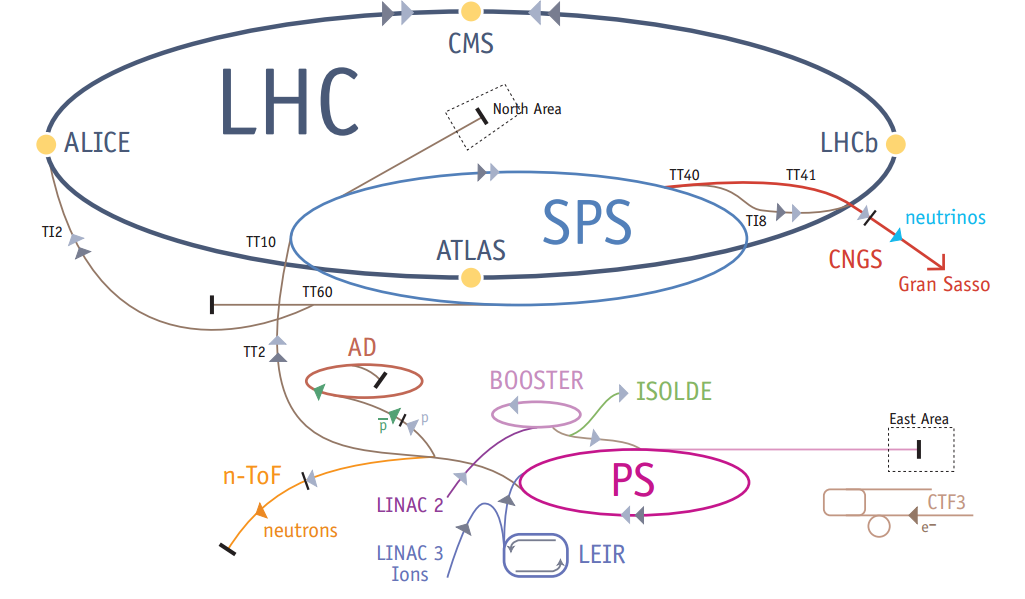
\includegraphics[width=0.95\textwidth]{lhc}
% 	\caption{Schematic of the \ac{LHC} accelerator complex \cite{lhc}.}
% 	\label{p18}
% \end{figure}
% % ========================================================
% % CMS
% % ========================================================
% \section{\acf{CMS}}
% \ac{CMS}, one of the general experiments at \ac{LHC}, is located beneath the French town Cessy. One of its main goals was the recent discovery of a new boson (assumed to be Higgs). Now the remaining  goals are the study of the properties of this boson and the search for evidence of physics beyond the Standard Model, in particular \ac{SUSY} and extra dimensions. The name \ac{CMS} derives from its design, which is rather small compared to other detectors of its capability (\ac{ATLAS}). \ac{CMS} has an excellent ability to measure myon tracks and a unique, very strong solenoid magnet.\\
% A sectional view of the whole detector is shown in \ar{p19}. It is set up in many shells of sub-detectors like layers of an onion. After the interaction, particles first pass the innermost detector, which is a tracker detector that measures i.a. the trajectory. After that comes an \ac{ECAL} and a \ac{HCAL} that measure the energy of the particles. The already mentioned sub-detectors are enclosed by the solenoid. The outermost layers outside of the coils consist of muon chamber. The \ac{CMS}-Pixel chip that is important for this thesis, is located in the innermost layer and is part of the tracker detector.
% \begin{figure}[ht]
% 	\centering
% 	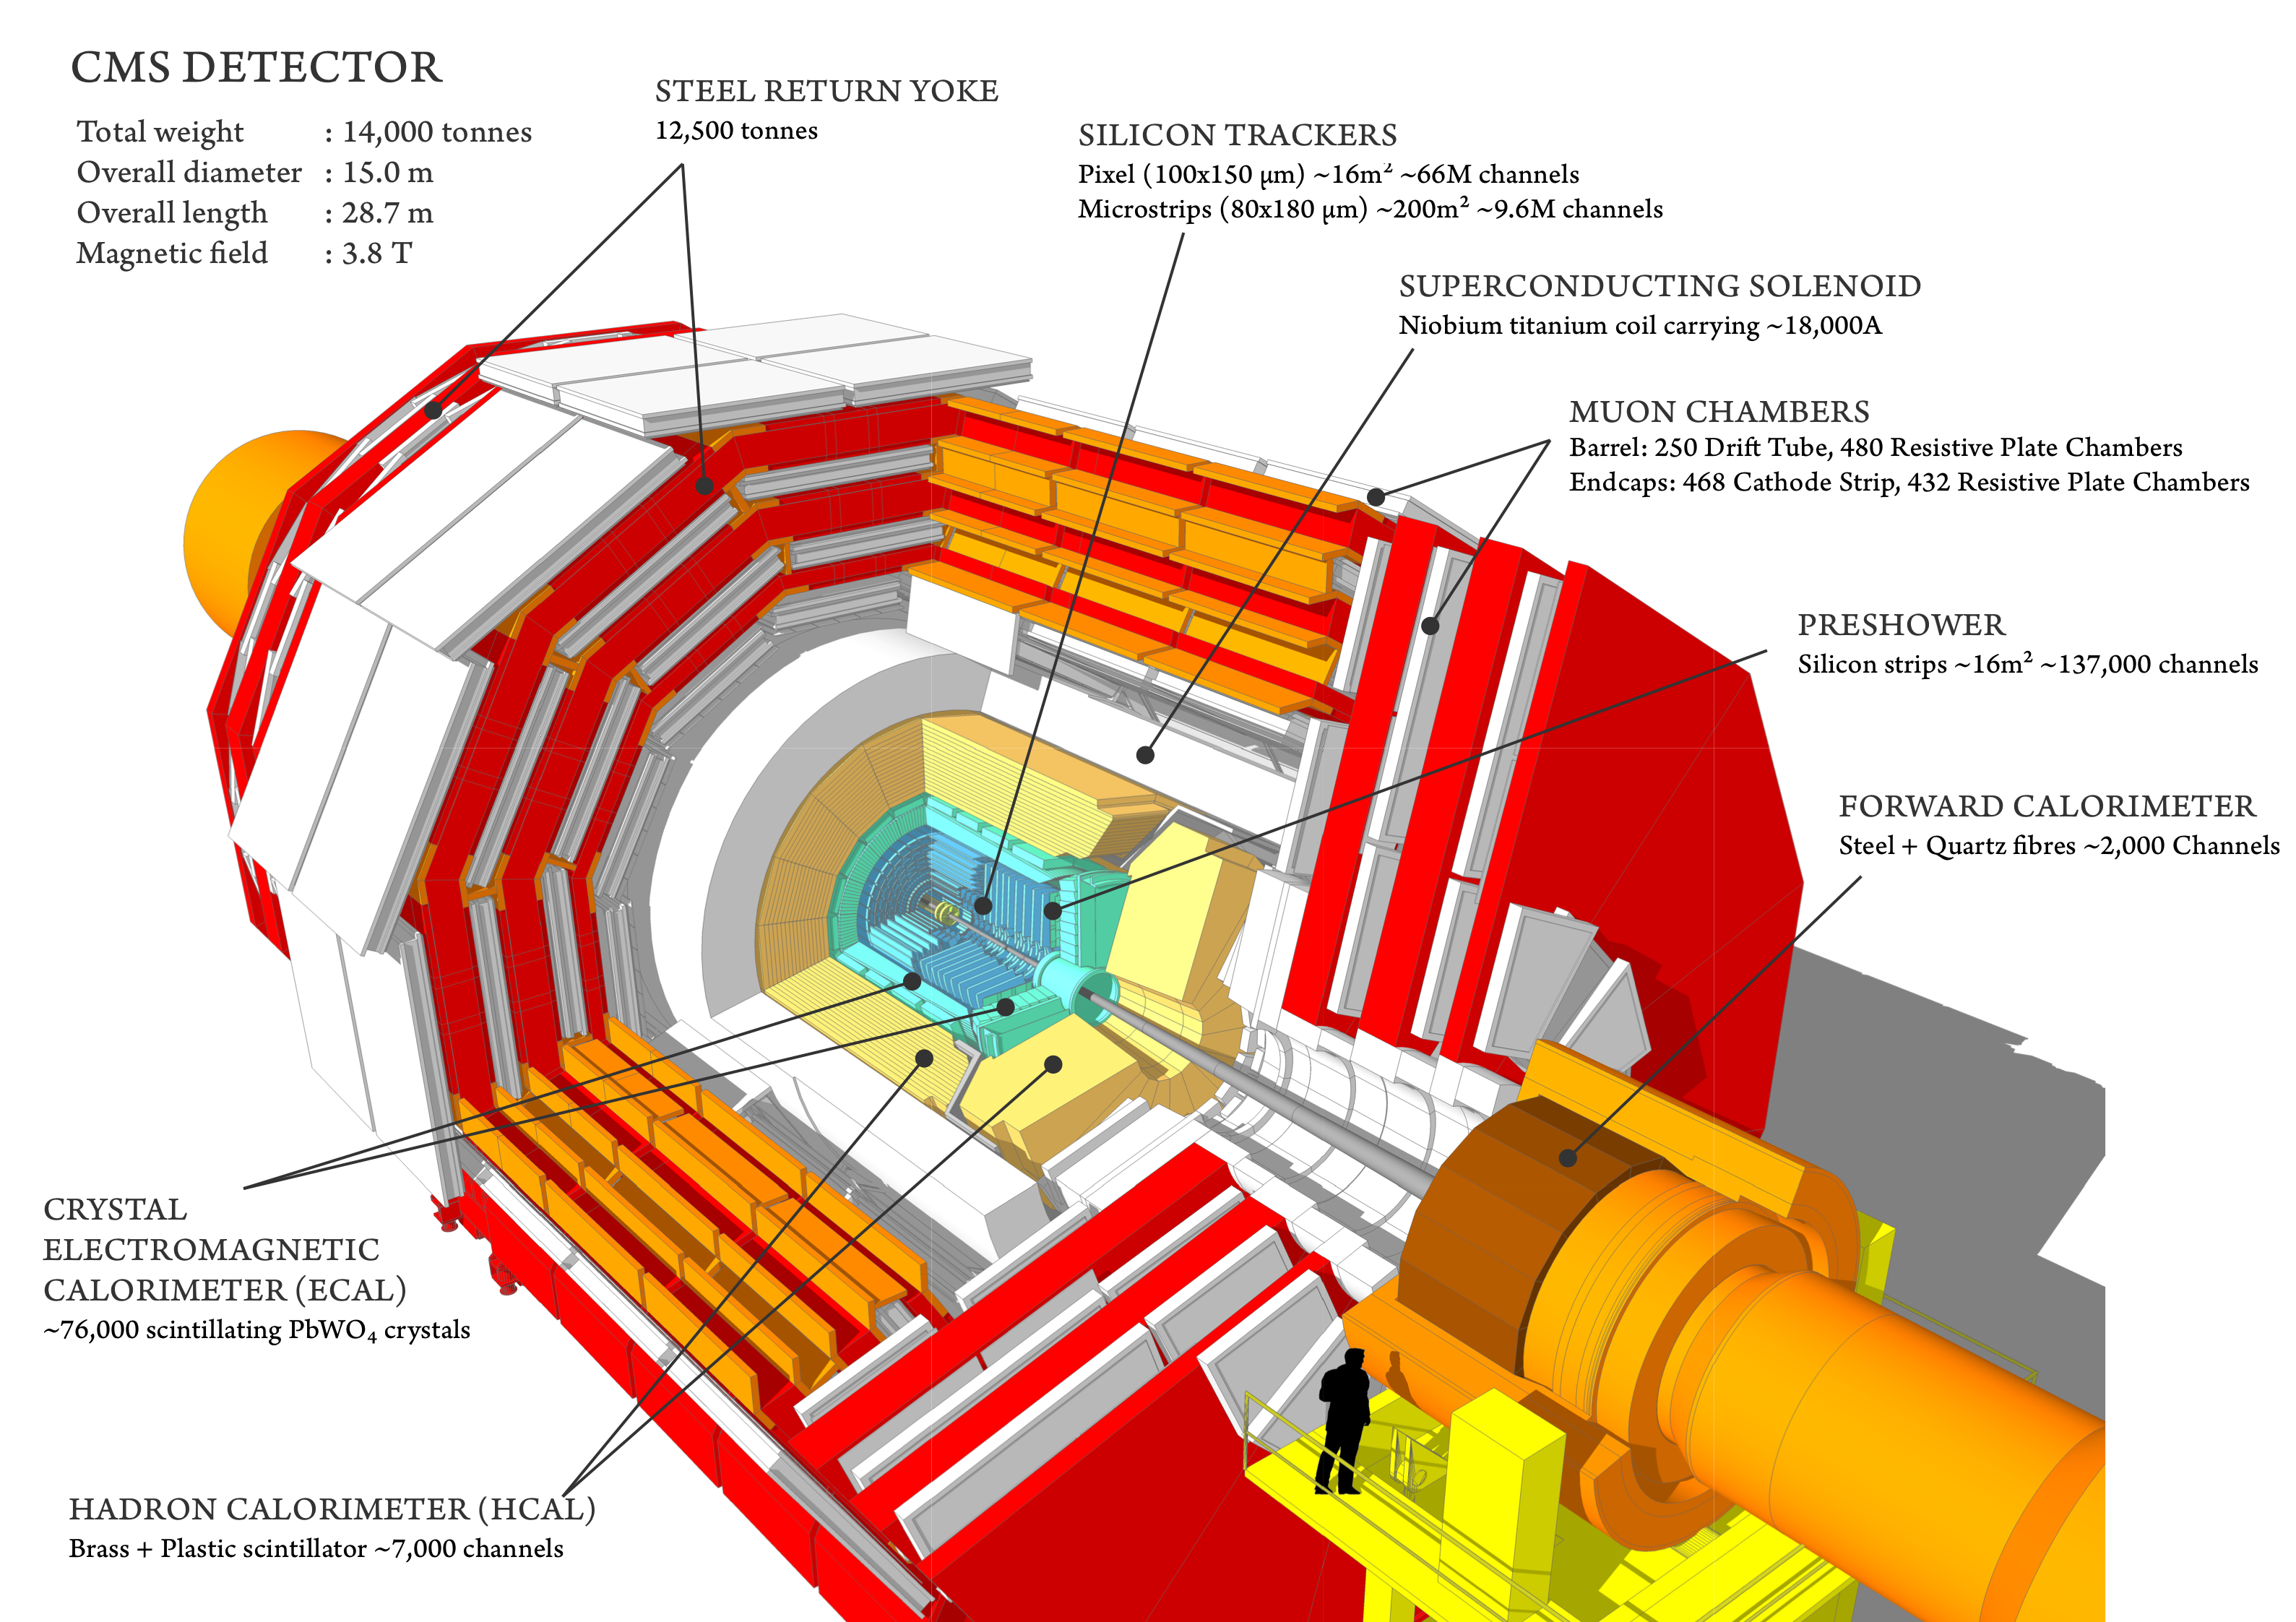
\includegraphics[width=0.95\textwidth]{cms_cut}
% 	\caption{Sectional view of the CMS detector \cite{cmsdet}.}
% 	\label{p19}
% \end{figure}
% % ========================================================
% \subsection{Solenoid}
% The shape of the solenoid strongly determines the whole design of the detector. A solenoid is a magnet of coils that are tightly wound into helices and have uniform magnetic field inside the helix, once constant electric current flows through the wires. Its purpose is to bend the paths of the particles that are created at the interaction point. It was aimed to be the strongest possible magnet since a stronger magnetic field leads to a smaller bending ratio of the particle gets and consequently increases the momentum resolution of the tracker. To reach a final magnetic field strength of $4\,$Tesla the whole magnet is cooled down to a temperature of $-268.5\,^{\circ}$C to guarantee superconductivity. Interestingly, particles with an energy of less than $1.6\,$GeV will circle inside the detector and will traverse to the end caps on a helical trajectory without ever reaching the calorimeter. 
% % ========================================================
% \subsection{Tracker Detector}
% The main goal of the tracker detector is to measure the momentum and the trajectory of passing particles to be able to get an idea of the incidents after the collision. The momentum is calculated using the circular trajectory of charged particles caused by the magnetic field. The \ac{CMS} tracker records the path of the charged particle by finding its position at a number of key points at each sub-layer of the detector. That way it is possible to precisely reconstruct paths of long living particles such as muons, electrons or hadrons, but also see the tracks of short living particles such as the beauty quark.\\
% For the whole experiment is very important to measure precise tracks on the one hand as well as to have as less disturbing\footnote{Less disturbing in that context means that the interactions of the Particles with the whole tracking detector has to be kept at a minimum.} of the particles as possible. That is one reason why only a certain number of points are measured for the tracking rather than than the maximum number. This was accomplished building $3$ layers of sub-tracker detectors around the beam line.\\
% The innermost layer of the detector is located but $4.4\,$cm away from the interaction point where the detectors are exposed to an approximate particle flux of $100\,$Mhz\,cm$^{-2}$. That is why the most important properties of the detector have to be radiation hardness and the ability to process a very high rate of events. When the current detector was built, it was decided to make it completely out of silicon. To be able to deal with the high number of particles the inner layers are made of pixel detectors whereas the outer ones, more than $20\,$cm away from the interaction point, are made out of strip detectors.
% % ==========================
% \subsubsection{Pixel Detector}
% Though only roughly the size of a shoe box, the Pixel Detector at \ac{CMS} contains $65$ million single pixels. They are arranged in three layers of barrel detectors $4.4\,$cm, $7.3\,$cm and $10.2\,$cm away from the beam and two forward detectors at either end (q.v. \ar{p22}). This system is able to reconstruct the tracks of ten million track per second and was build to withstand the duration for an operation time of ten years up to the Phase 1 Upgrade. Due to the huge amount of pixels it important keep the power consumption of the \ac{ROC}s at a minimum. Although they only need $50\,\upmu$W per pixel they are still mounted on cooling tubes so that the detector will not overheat. The cooling is also important reduce the electronic noise.\\
% The \ac{CMS} Pixel Detector is also the most important part concerning my thesis and is explained in further detail in \ar{s130}.
% \begin{figure}[ht]
% 	\centering
% 	\subbottom[\ac{CMS} silicon pixel detector \cite{cmsweb}.\label{p21}]{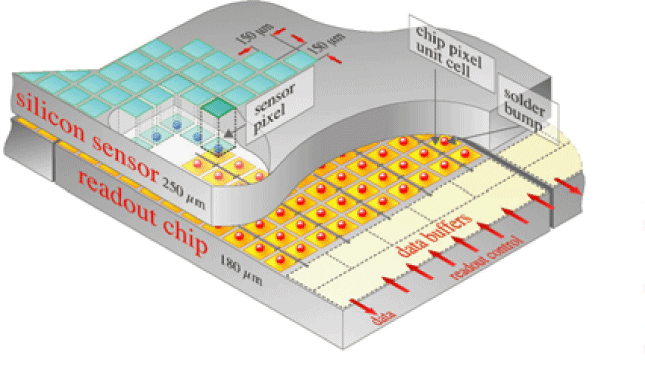
\includegraphics[width=0.47\textwidth]{pixelement}}
% 	\hfill
% 	\subbottom[Pixel layers around the beam line \cite{bora}.\label{p22}]{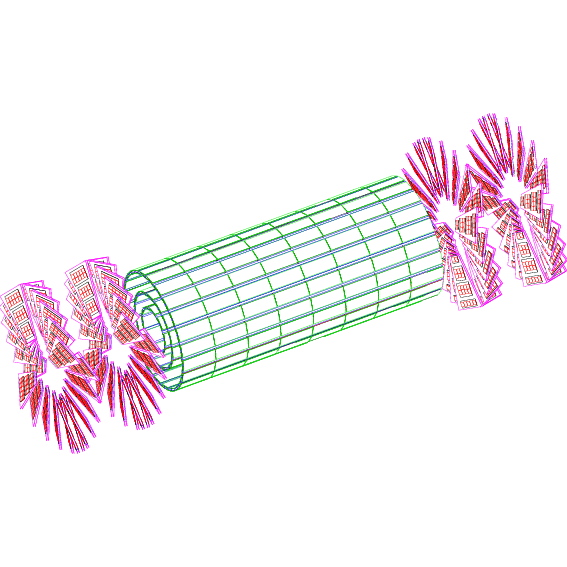
\includegraphics[width=0.47\textwidth]{barrel}}
% 	\caption{Schematics of the pixel detector.}
% 	\label{ppixdet}
% \end{figure}\no
% % ==========================
% \subsubsection{Strip Detector}
% Ten layers of strip detectors up to a radius of $130\,$cm surround the three pixel layers. A schematic of the way strip detectors are placed around the beam line is shown in \ar{p23}. First come four inner barrel layers with two inner endcaps. After them follow the outer layers: two double sided and four one sided barrel layers. Altogether the tracker detector consist of $10$ million silicon strips, which have the same working principle as the pixel detectors even though different chips are used for the readout. The whole system is also cooled down, in this case to a temperature of $-20\,^{\circ}$C.
% \begin{figure}[ht]
% 	\centering
% 	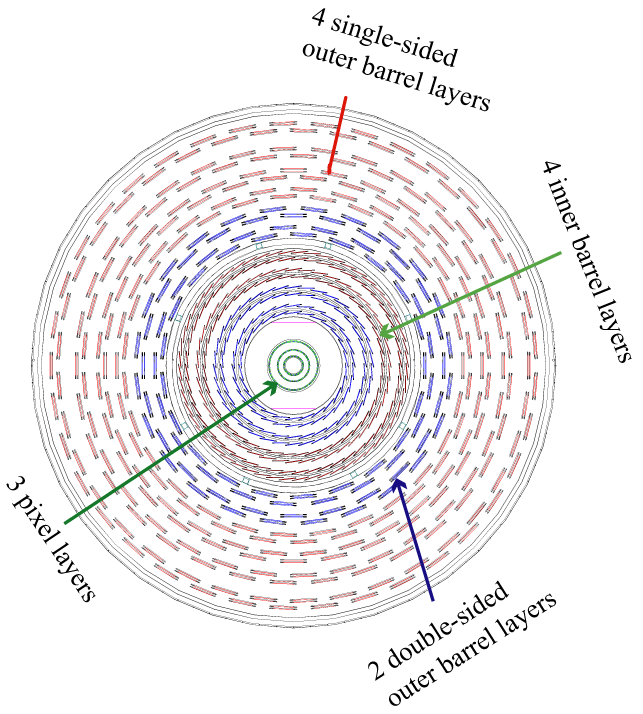
\includegraphics[width=0.4\textwidth]{strip}
% 	\caption{Tracker layers perpendicular to the beam \cite{cmsweb}.}
% 	\label{p23}
% \end{figure}
% % ========================================================
% \subsection{Calorimeter}
% In particle physics a calorimeter is a device to measure the energy of particles. When a particle enters the detector material a chain reaction called particle shower is started until the incident particle has deposited all its energy in the calorimeter. In many cases the detectors have transverse segmentation to provide information about the direction of the particle and longitudinal segmentation to get information about the identity of a particle by the shape of the shower. Since electrons and photons interact very differently with matter compared to hadrons, two different types of calorimeters are required: the \ac{ECAL} and the \ac{HCAL}.
% % ==========================
% \subsubsection{\ac{ECAL}}
% The \ac{ECAL} consists of $75848$ lead tungstate crystals (\chemfig{PbWO_{4}}), which is a scintillating material. With a short radiation length, narrow showers and a good radiation hardness \chemfig{PbWO_{4}} has excellent properties to function in such an environment. Glued on top of the crystals are photodetectors that collect the light, amplify it and transform it into into a electric signal, which then can be analysed.
% % ==========================
% \subsubsection{\ac{HCAL}}
% The \ac{HCAL} is built to measure hadrons which consist out of quarks and gluons. It was designed to be as hermetic as possible, i.e. to stop every particle from the collision in order to be able to draw conclusions about missing transverse energy. It is a so called sampling calorimeter which means that it finds the position, energy and arrival of a particle by using repeating layers of a dense brass absorber and plastic scintillators. This repeating architecture is also called sandwich structure. The \ac{HCAL} is the last part of the detector that is placed inside the solenoid.
% % ========================================================
% \subsection{Muon Chambers}
% Arranged on the outside of the solenoid are the muon chambers, since muons can even penetrate very dense material without losing a lot of energy. They are produced as decay products of many particles including potential new ones and thus play an import role as signals that can be triggered on. The whole muon detector consists of $1400$ muon chambers that split up into $250$ drift tubes and $540$ cathode strip chambers that track the particles and provide a trigger. The other part are $610$ resistive plate chambers that form a redundant trigger system, which decides weather to keep the data or not.
% % ========================================================
% \subsection{Examples}
% A diagram of all parts and the positioning within the \ac{CMS} detector is shown in \ar{p20}. It also demonstrates how typical particles will behave passing through the various steps. Photons and electrons are both stopped in the \ac{ECAL} but due to their charge electrons show a curved path in the tracker whereas photon tracks are straight. Charged hadrons will also leave a curved track and are generally stopped in the \ac{HCAL}. Because most myons are \ac{MIP}s they will not stop at all, but show a double curved track due the opposite magnetic field on the outside of the Solenoid.
% \begin{figure}[ht]
% 	\centering
% 	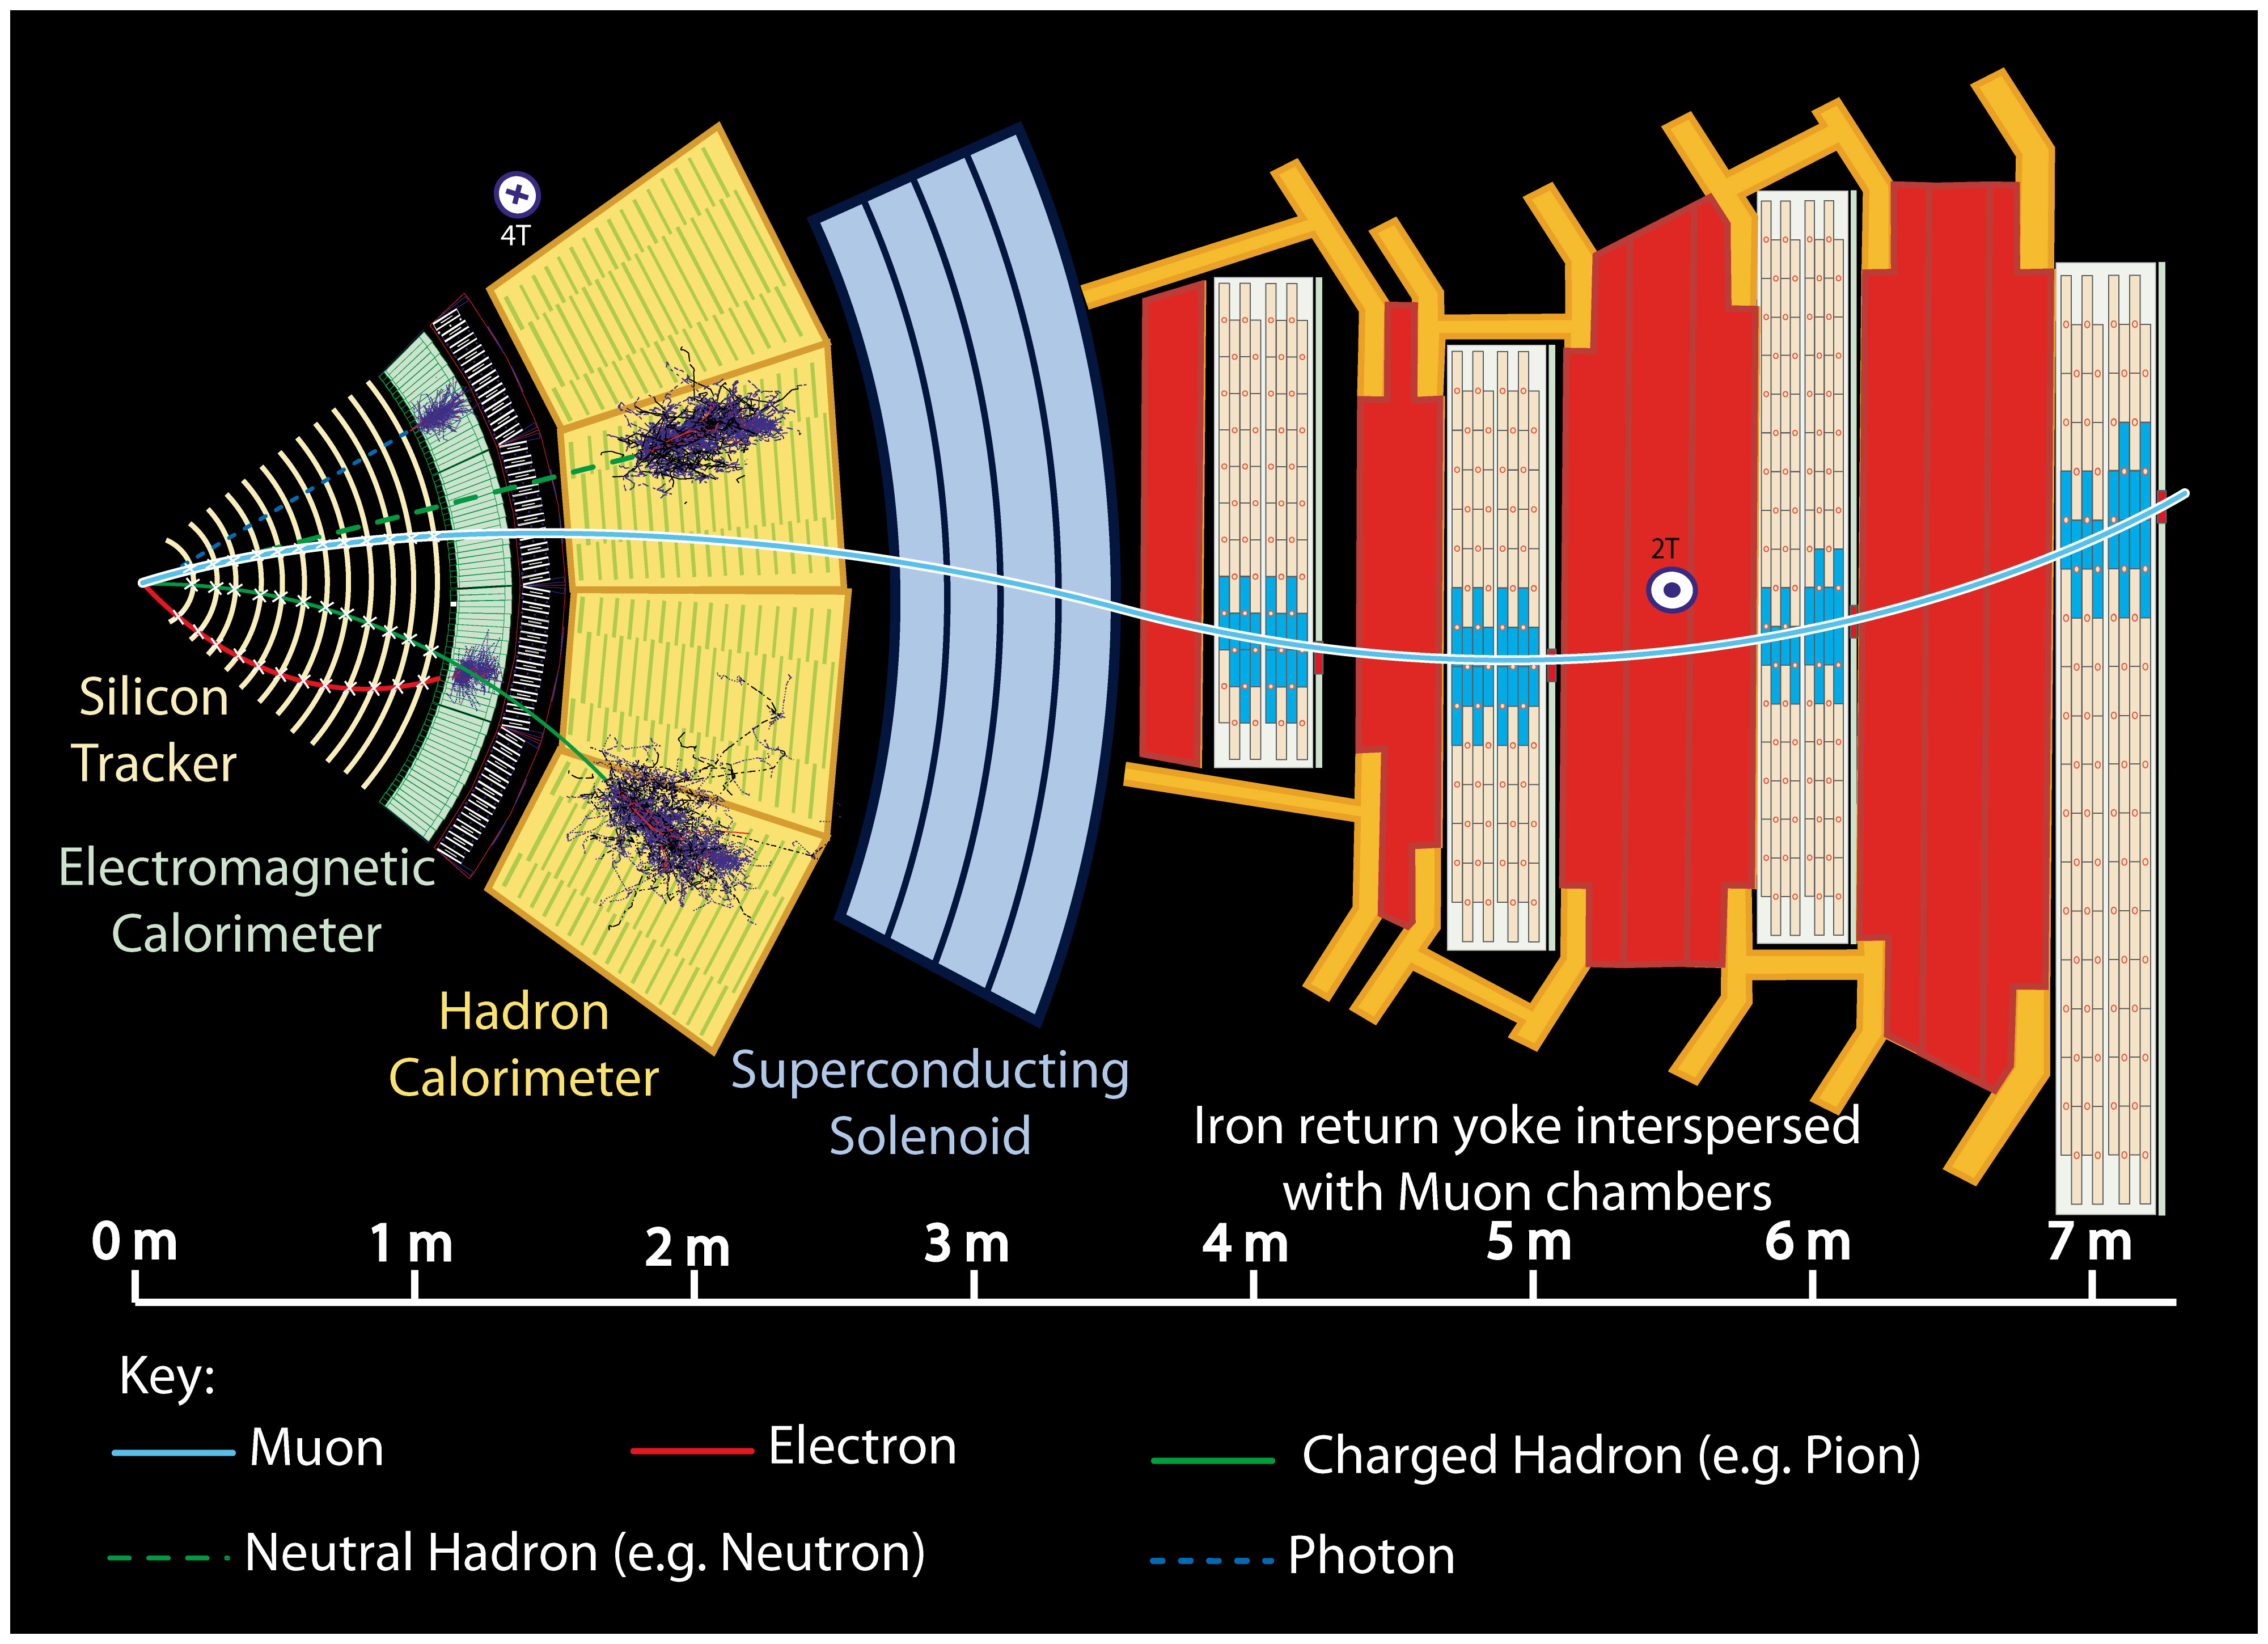
\includegraphics[width=0.95\textwidth]{cms_slice}
% 	\caption{Sliced view of the CMS detector with tracks of various particles \cite{cmsweb}.}
% 	\label{p20}
% \end{figure}
% % ========================================================
% \subsection{Trigger System}
% With almost a billion interactions per second\footnote{Roughly $20$ interactions per collision at a rate of $40\,$Mhz add up to a billion interactions} it is almost impossible to save or even analyse every single event. That is why a trigger system is required to save only the interesting events. Since there are collisions every $25\,$ns the data is stored in pipelines with precise timing information for a short time. In order not to mix up information from different events it is very important to synchronise the data streams. \\
% The first step to reduce the huge amount of information happens through the level 1 trigger, which is a full hardware trigger that decides within $3.2\,\upmu$s if the event could contain interesting physics based on information of the calorimeter and the muon chambers. These are events with large amount of energy or unusual combination of particles for example. The level 1 trigger selects $100\,$kHz of events out of the $1\,$GHz that are available. In the next step, the high level trigger, the whole event is recreated and the information sent to computers to pre-analyse it, which makes it a full software trigger. In the end only $100$ events per second are considered interesting and will be saved.\\ 
% The delays and the principle of the level 1 trigger of \ac{CMS} is important because it has direct connection to the trigger system used in the experiments concerning this thesis. 
% % ========================================================
% % CMS Pixel Chip
% % ========================================================
The CMS pixel chip is a tiny part of a detector of the world's most powerful high energy particle accelerator, the \ac{LHC}. It is utilised in the innermost layers of the tracker detector of \ac{CMS}, one of the two general purpose experiments at the \ac{CERN}. There it is essentially used to reconstruct particle tracks and measure the momenta of the charged particle using the tracks. The whole \ac{CMS} pixel detector is based on the pixel chip psi46v2 which has an analogue readout. During the Phase 1 Upgrade it is planned to exchange all of them with a more efficient digital silicon chip. It was also decided to add a fourth layer to the pixel detector. Due to the increase of the luminosity and \ac{COM} energy the Phase 2 Upgrade will require different materials for the innermost layers. A potential candidate are diamond pixel chips. Among other advantageous properties diamond is much more radiation resistant than silicon. Though, if diamonds are suited for that purpose is still under test.\\
During this thesis both analogue and digital silicon chips were used and there even was an opportunity to test digital diamond pixel chips. The purpose for the conducted experiments is in parts the exact same as for \ac{CMS}: use several \ac{ROC}s as tracking device. Additional applications will be described in the following.
% ========================================================
\section{Analogue Pixel Detector}\label{s130}
The analogue pixel detector was designed, inter alia, to precisely reconstruct hits, withstand radiation damage for several years of operation, keep multiple scattering at a minimum and avoid fake hits due to noise in electronics. Each single chip consists out of $4160$ pixels in $26$ double columns and $80$ rows. The single pixels have a size of $150\,\upmu$m $\times$ $100\,\upmu$m, which adds up to a total size of $7.8\,$mm $\times\ 8.0\,$mm (q.v. \ar{p24}) and corresponds to an area of a little more than half a square centimetre. The detector itself consists of two parts: a pixelated silicon sensor and a \ac{ROC}, which have both the same arrangement of pixels. The bump bonds are schematically shown in \ar{pbumpbonds} They are attached to one another and electrically connected via indium bump bonds of roughly $20\,\upmu$m in diameter \cite{kaestli}. The connection from the \ac{ROC} to the readout as well as the connection to the bias voltage is made via delicate wire-bonds.
\begin{figure}[ht]
	\centering
	\subbottom[Principle of a sensor bump bonded to the a chip \cite{dectris}.]{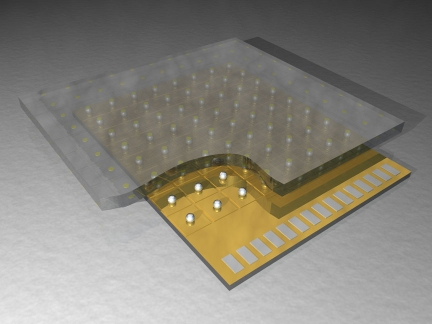
\includegraphics[width=0.47\textwidth]{bumpbonds}\label{pbumpbonds}}
	\hfill
	\subbottom[Photograph of an analogue pixel detector. The wire bonds are visible in the top right corner]{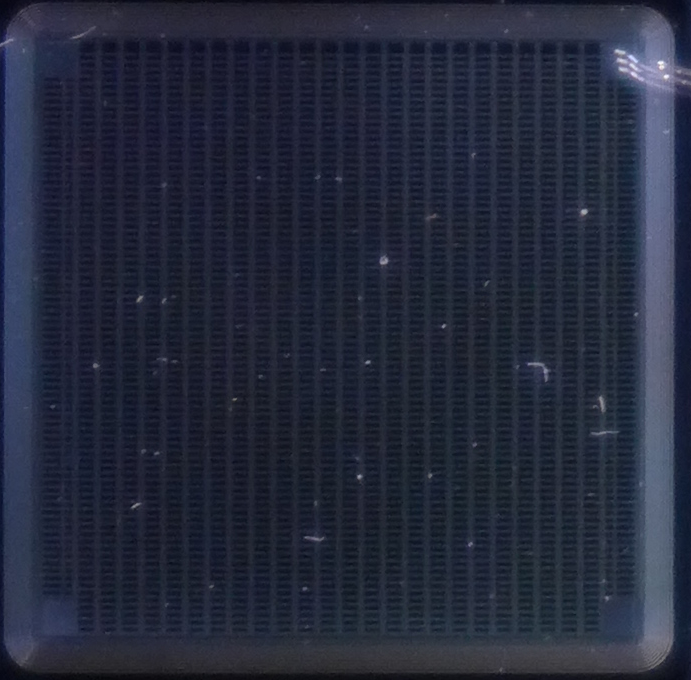
\includegraphics[width=0.47\textwidth]{ROC0}\label{p24}}
	\caption{Parts of the pixel detector.}
	\label{panaroc}
\end{figure}\no
% =======================
\subsection{Sensor}\label{s220}
For the current detector silicon was chosen as sensor material. The average energy to create an electron-hole pair in silicon is $3.6\,$eV. By applying a bias voltage to the sensor the charge carriers are moved to the collecting electrode and a signal can be measured. The silicon sensor itself consists of high-dose n-implanted pixels introduced into a high resistive n-substrate. The backside of the sensor is p-doped and thus creates a pn-junction \cite{allkofer}. The small pixel size was chosen to get a good spatial resolution. The thickness of the sensor is about $285\,\upmu$m so that minimum ionising particles will most probably create approximately $22000$ electron-hole pairs\footnote{The energy is loss is Landau distributed. This value is equivalent to the peak value of this distribution (q.v. \ar{slandau})} in the sensor. In order to fully deplete an unirradiated sensor of that thickness completely one has to apply a bias voltage of roughly $100\,$V \cite{pixadd}. For irradiated detectors that value may be a couple times higher, depending on the irradiation damage. 
% =======================
\subsection{\acs{ROC}}\label{sroc}
The \ac{ROC} has two parts: An active part consisting out of $26$ double columns of $2\times80$ \ac{PUC}s matching the pixels of the sensor and a periphery consisting of a control interface block, a data buffer, a time-stamp buffer and $35$ supply pads; this is depicted in \ar{p8}. All the signals going to and coming from the \ac{ROC} are put on these supply pads.\\
In order for the \ac{ROC} to record data, handle triggers and manage the readout, it also has four different counters:
\begin{enumerate}
	\item An $8\,$bit bunch crossing counter - whose information is sent to the time-stamp buffer,
	\item an $8\,$bit bunch crossing counter with trigger delay - runs a number of counts behind the bunch crossing counter (adjustable by the \ac{DAC} value wbc),
	\item an $4\,$bit trigger counter,
	\item an $4\,$bit token counter.
\end{enumerate}\par
The periphery is the reason is why the \ac{ROC} is with $7.9\,$mm$\times\ 9.8\,$mm 
\begin{wrapfigure}{l}{7.2cm}
	\vspace*{-10pt}
	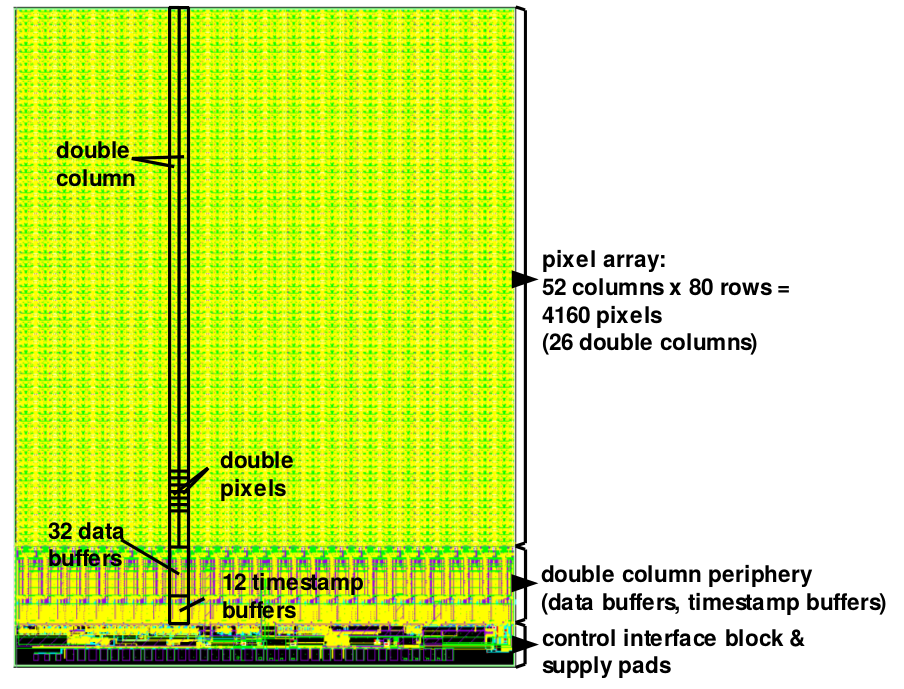
\includegraphics[width=7.2cm]{ROC_scheme}
	\caption{schematics of a \ac{ROC} \cite{psi46chip}}
	\label{p8}
	\vspace*{-5pt}
\end{wrapfigure}  
a few millimetres longer than the pixelated area of the sensor. The \ac{ROC} is programmable with a set of  $26$ \ac{DAC} values (q.v. \ar{t0}) that are required to control its behaviour. More details about the \ac{DAC}s can be found in \ar{sdacs}. The \ac{ROC} and its behaviour is temperature dependent, which is why it is also equipped with a temperature sensor.\\
If electron-hole pairs are created in the sensor, a voltage signal is induced in the corresponding \ac{PUC}. A schematic of a \ac{PUC} is shown in \ar{p9}. Once a signal enters the \ac{PUC} it gets amplified and shaped. If it exceeds a certain threshold, which is tunable with one the \ac{DAC}s, a signal is immediately sent to the periphery that will save the current bunch crossing into the time stamp buffer. The information of the hit (the \ac{PUC} address and the \ac{PH}) will be sent to a sample and hold capacitance until it is read out, which happens every $25\,$ns. Once read out, the data is stored in the data buffer.\\ 
There is an option to sent calibration signals directly to the front end of the \ac{PUC} that makes it very easy to test the basic functionality of the \ac{ROC} without requiring any particle hits. For every pixel the \ac{PUC} has a register to enable and disable sending these calibrates.\\
Furthermore, an important feature of the analogue \ac{ROC} is the so called fast-OR. Every time the threshold of a single pixel is exceeded, the \ac{ROC} sends out this signal. It is an logical OR of all pixels of the \ac{ROC} and its shape gives, inter alia, conclusions about the distribution of hit pixels (q.v. \ar{sfastor}). It is very important as trigger signal for other devices or as self trigger.
\begin{figure}[ht]
	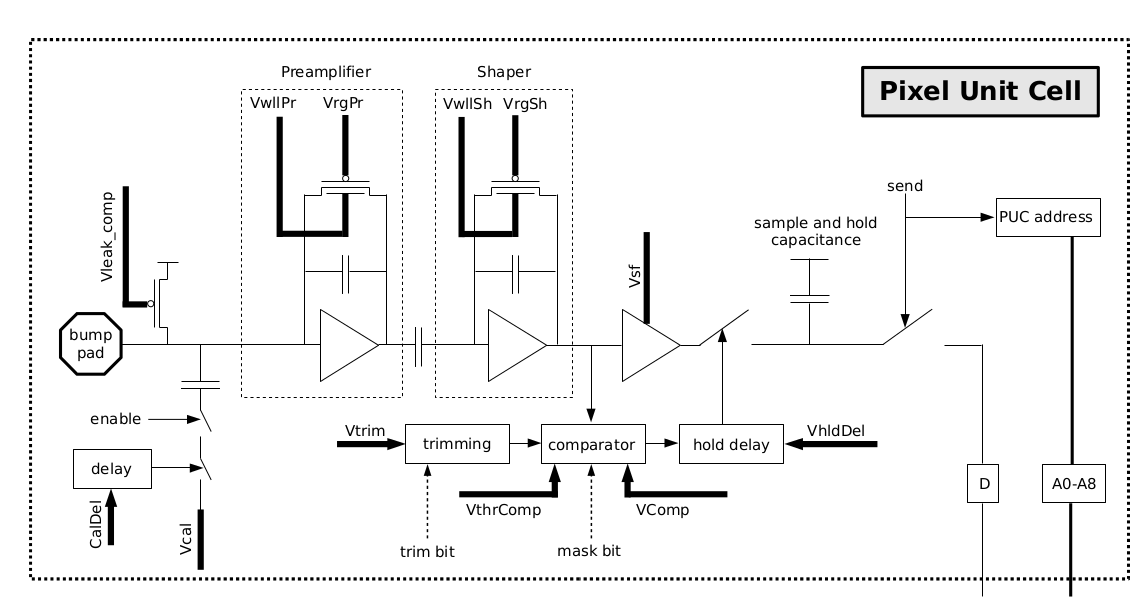
\includegraphics[width=0.95\textwidth]{PUC}
	\caption{Schematic view of a \ac{PUC} \cite{dambach}.}
	\label{p9}
\end{figure}
% =======================
\subsection{\acs{DAC}s}\label{sdacs}
An overview of all existing \ac{DAC}s for the analogue pixel chip with a short explanation is shown in \ar{t0} and \ar{t2}. In the following the most important \ac{DAC}s concerning this thesis are named.\\
In order to operate the chip it has to be supplied with a voltage. It was found that the chip is showing the best results while operating at a stable analogue current of $24\,$mA \cite{dambach}. This current can be adjusted by the $8\,$bit \ac{DAC} \textit{vana}. To be able to do basic tests with calibrate signals the correlation between \textit{vthrcomp} and \textit{caldel} has to be taken into account. It is only working in a certain region, which is explained in more detail in \ar{stornado}. Furthermore a common threshold for all pixels is of great importance. To achieve this a process called trimming is applied that exploits the inverse \ac{DAC} \textit{vthrcomp} and the \ac{DAC}s \textit{vcal} and \textit{vtrim}. More information about the trimming can be found in \ar{strim}. \textit{Vthrcomp} sets the global comparator threshold and \textit{vtrim} is responsible for the amount this global threshold can be lowered for each pixel. \textit{Vcal} regulates the amplitude of the calibrate signal and can be converted to the number of electrons created in the sensor. That is why it is also used to set a value for the common threshold.\\
Since for the undertaken experiments it was most important to have a stable fast-OR, \textit{vicolor}, \textit{vnpix} and \textit{vsumcol} were set in a way to have the maximum amplitude of the signal regardless of the shape. More details about the fast-OR and the effect of these \ac{DAC}s are in \ar{sfastor}.\\
\textit{Phoffset} and \textit{vcomp\_adc} can be used to adjust the address levels of the \ac{ROC}.
\begin{table}[ht]
	\begin{tabularx}{\textwidth}{c|l|X}
		\noalign{\hrule height 2pt}
		\textbf{\#} & \multicolumn{1}{c}{\textbf{Name(s)}} & \multicolumn{1}{|c}{\textbf{Explanation}}	\\\noalign{\hrule height 2pt}
		\multicolumn{3}{c}{\textbf{Voltage regulators}}														\\\hline
		$01$ & 	vdig				& sets the digital current 												\\\hline
		$02$ &	vana				& sets the analogue current 											\\\hline
		$03$ &  vsf // vsh			& influence on pulse height in low vcal range and digital current		\\\hline
		$04$ & 	vcomp				& regulates the supply voltage of the comparator						\\\noalign{\hrule height 2pt}
		\multicolumn{3}{c}{\textbf{Analogue Signal (\ac{PUC})}}												\\\hline
		$05$ &	vleak\_comp // vleak& controls leakage current 												\\\hline
		$06$ &	vrgpr				& \multirow{4}{7.6cm}{together control the pre-amplifier and the shaper and thereby the shape of the incoming signal}\\
		$07$ &	vwllpr				& 			 															\\
		$08$ &	vrgsh				& 																		\\
		$09$ &	vwllsh				&																		\\\hline
		$10$ &	vhlddel				& slightly influences the pulse height for different \textit{vcals} and pixels	\\\hline
		$11$ &	vtrim				& defines how much the trim bits for each pixel will increase the threshold\\\hline
		$12$ &	vthrcomp			& global comparator threshold											\\\noalign{\hrule height 2pt}
		\multicolumn{3}{c}{\textbf{Fast-OR Trigger (\ac{PUC})}}												\\\hline
		$22$ &	vicolor 			& \multirow{3}{7.6cm}{together define the shape of the fast-OR signal}		\\
		$23$ &	vnpix 				&  																		\\
		$24$ &	vsumcol	 			&  																		\\\noalign{\hrule height 2pt}
		\multicolumn{3}{c}{\textbf{Calibrate Signal (\ac{PUC})}}											\\\hline
		$22$ &	vcal	 			& sets the voltage for the calibrate signal (two ranges) 				\\\hline
		$22$ &	caldel	 			& delay of the calibrate signal											\\\noalign{\hrule height 2pt}
		\multicolumn{3}{c}{\textbf{Double Column Periphery}}												\\\hline
		$13$ &	vibias\_bus 		& switch for sending the address of the \ac{PUC} 						\\\hline
		$14$ &	vbias\_sf			& shifts the pulse height curve 										\\\hline
		$15$ &	voffsetop			& shift of pulse height  												\\\hline
		$16$ &	vibiasop			& switch for pulse height and influence of linear range 				\\\hline
		$17$ &	voffsetroc // phoffset	& switch for pulse height and influence of linear range 			\\\hline
		$18$ &	vion				& scaling of the pulse heights 											\\
		\noalign{\hrule height 2pt}
	\end{tabularx}					
	\caption{\ac{DAC}s of the pixel chip \cite{dambach}. Some \ac{DAC}s were renamed during the evolution of the chip which is why one \ac{DAC} can have several names.}
	\label{t0}
\end{table}\no
% =======================
\begin{table}[ht]
	\begin{tabularx}{\textwidth}{c|l|X}\noalign{\hrule height 2pt}
		\multicolumn{3}{c}{\textbf{Control and Interface Block}}											\\\hline
		$19$ &	ibias\_dac // vcomp\_adc	& scaling of the \ac{ROC} address levels and the pulse height 	\\\hline
		$20$ &	vibias\_ph // phscale& scaling of the pulse height 											\\\hline
		$21$ &	vibias\_roc 			& scaling of the \ac{ROC} address levels and the pulse height 		\\\noalign{\hrule height 2pt}
		\multicolumn{3}{c}{\textbf{Registers}}																\\\hline
		$253$ &	ctrlreg 			& switch between low and high vcal range (bit 2), full and half readout speed (bit 0) and on/off of the whole \ac{ROC} (bit 1)\\\hline
		$254$ &	wbc		 			& sets the bunch crossing at which the data will be read out 			\\\hline
		$255$ &	rangetemp 			& switch for different ranges of the temperature sensor  				\\\noalign{\hrule height 2pt}
	\end{tabularx}					
	\caption{\ac{DAC}s and Registers of the pixel chip \cite{dambach}}
	\label{t2}
\end{table}\no
% =======================
\subsection{Readout \& Trigger}\label{sread}
Each \ac{ROC} is set up to be read out in zero suppression mode, which means that only for pixel hits that exceed the threshold, the following information is sent to the periphery: The time stamp of the current bunch crossing is written into the time stamp buffer and the analogue signals are written into the next free data buffer. This process happens autonomously and asynchronously for every double column.\\
Concerning the readout of the \ac{ROC} two external signal lines are of importance: The \ac{CTR} and the token. As the name suggests, the former can send three kinds of information depending on the length of the pulse:
\begin{enumerate}
	\item a trigger signal, which is two clock cycles long.
	\item a calibrate signal, which is one clock cycle long.
	\item a reset signal, which is three clock cycle long.
\end{enumerate}
The information in the \ac{ROC} data buffer has to be kept until a potential trigger arrives. They are stored in the data buffer until one of the following events happens: 
\begin{itemize}
	\item The data was successfully read out by a connected device.
	\item The trigger window is exceeded (the bunch crossing counter passes the delayed time-stamp).
	\item The data buffer is full.
	\item A reset signal was received.
\end{itemize}
The process of the readout is described in the following: Hits that were sent to the periphery are validated by the external trigger signal by comparing their corresponding time stamps with the delayed bunch crossing counter. Non-validated hits are cleared. If the validation succeeds, the trigger counter is latched into the periphery, i.e. the double column is frozen and will not record further data until the information is read out or the \ac{ROC} receives a reset signal. Other double columns without validated hits remain active. When the latched trigger counter is matching the token counter the double column is set to readout mode and the trigger counter is incremented. As soon as the \ac{ROC} receives a token the frozen double columns are read out and reset. A token sent to the \ac{ROC} travels along the periphery consecutively reading out frozen \ac{DC}s. Just before the token leaves the periphery of a \ac{DC}, the token counter of that column is incremented as well. To every readout of the $26$ \ac{DC}s the \ac{ROC} also adds a header. Illustrations of the trigger validation and the readout procedure are shown in \ar{pro}.
\begin{figure}[ht]
	\centering
	\subbottom[Trigger validation.]{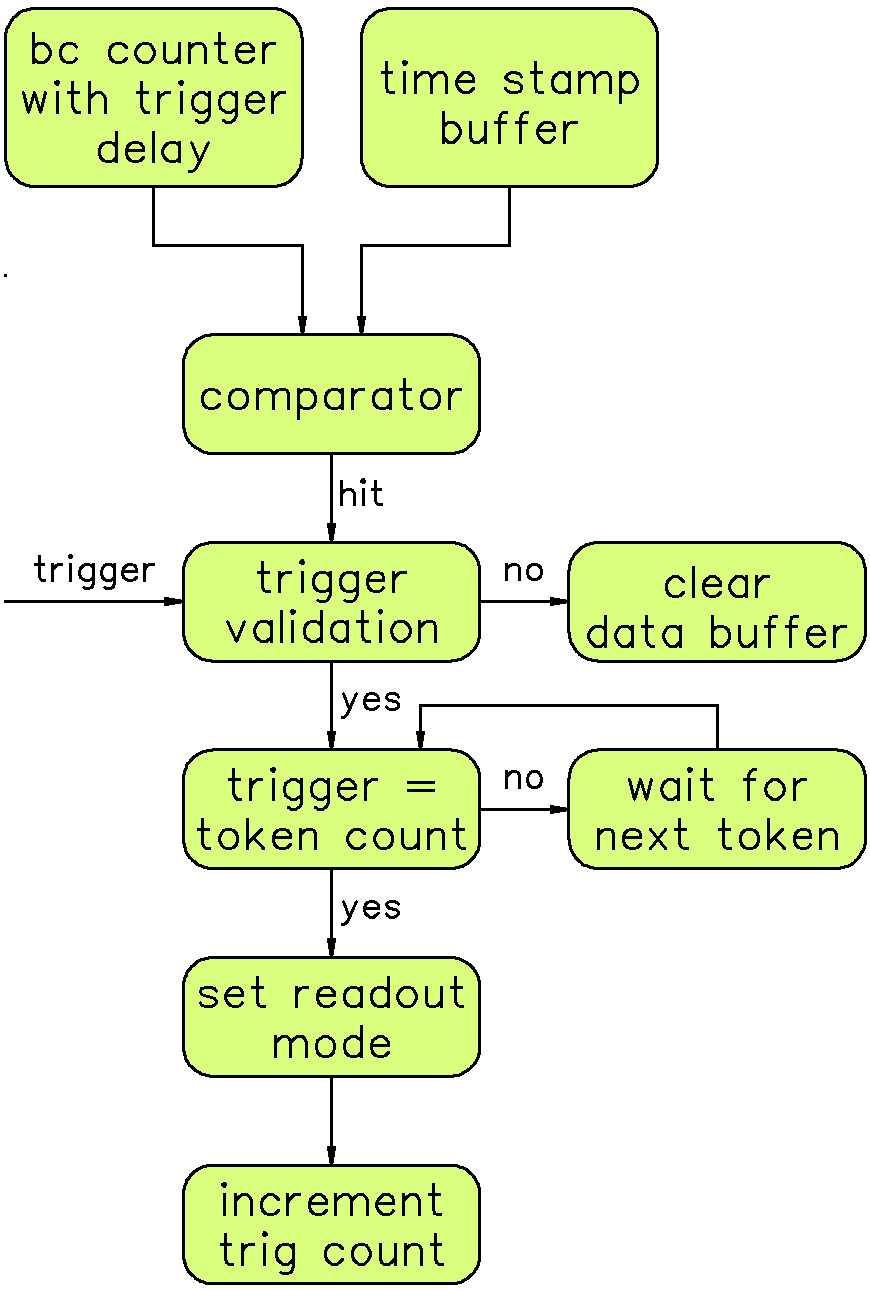
\includegraphics[width=0.37\textwidth]{trigger}\label{ptrig}}
	\hfill
	\subbottom[Readout procedure.]{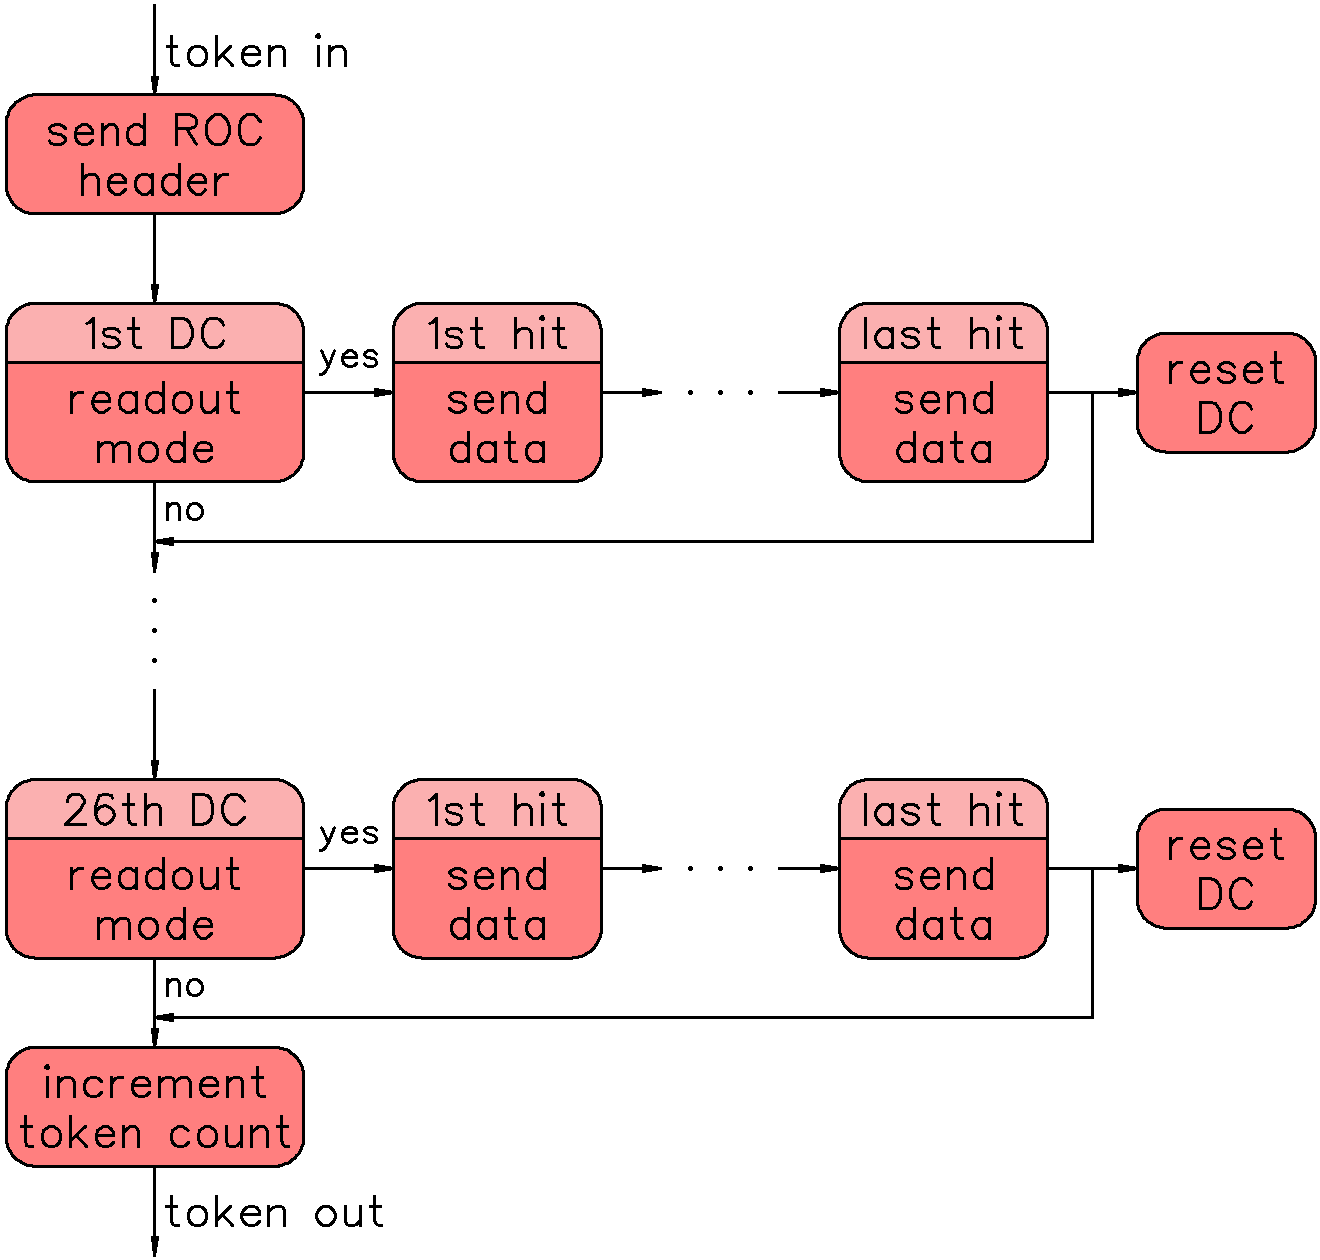
\includegraphics[width=0.57\textwidth]{token}\label{ptok}}
	\caption{Schematics of the readout of the \ac{ROC}. bc is short for bunch crossing and DC stands for double column}
	\label{pro}
\end{figure}\no
% =======================
\subsection{Data Format}\label{sdata}
An example of an analogue readout with only the information of the \ac{ROC} is shown in \ar{procsig}. The \ac{ROC} header is three clock cycles long. It contains an \ac{UB} level that is a very low, negative level and serves as reference, a \ac{B} level that is the zero reference of the differential signal and a level that is called \ac{LD}. The latter either points to the value the last \ac{DAC} was set to or the value of the temperature sensor of the chip. For every single pixel that was hit the \ac{ROC} will provide five levels containing the pixel address and one level with information about the pulse height. These six level are added to the header for each hit pixel. If no pixel was hit or the hits were not validated, the \ac{ROC} will send nothing but a header if a readout is started.\\
It is possible to read out several \ac{ROC}s with a single token. In that case the token is sent from one \ac{ROC} to the next collecting a header of each \ac{ROC} and the corresponding hit information s.t. a structure like header/hit/header/hit/hit/header/header/hit etc. will form. The readout concerning sending and handling trigger, reset and token is managed by a \ac{TBM}. For all the experiments described in the thesis the data was read with a \ac{DTB} that was developed at \ac{PSI}. The \ac{DTB} utilises a \ac{TBM} emulated on its \ac{FPGA} and is described in more detail in \ar{sdtb}.\\
\begin{figure}[ht]
	\centering
	\subbottom[Measured signal of several single pixel hits.\label{panasig}]{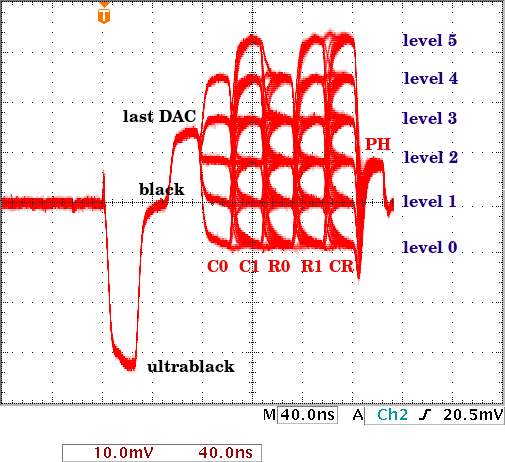
\includegraphics[width=0.47\textwidth]{siganalog}}
	\hfill
	\subbottom[Schematic signal of one single pixel hit.\label{p7}]{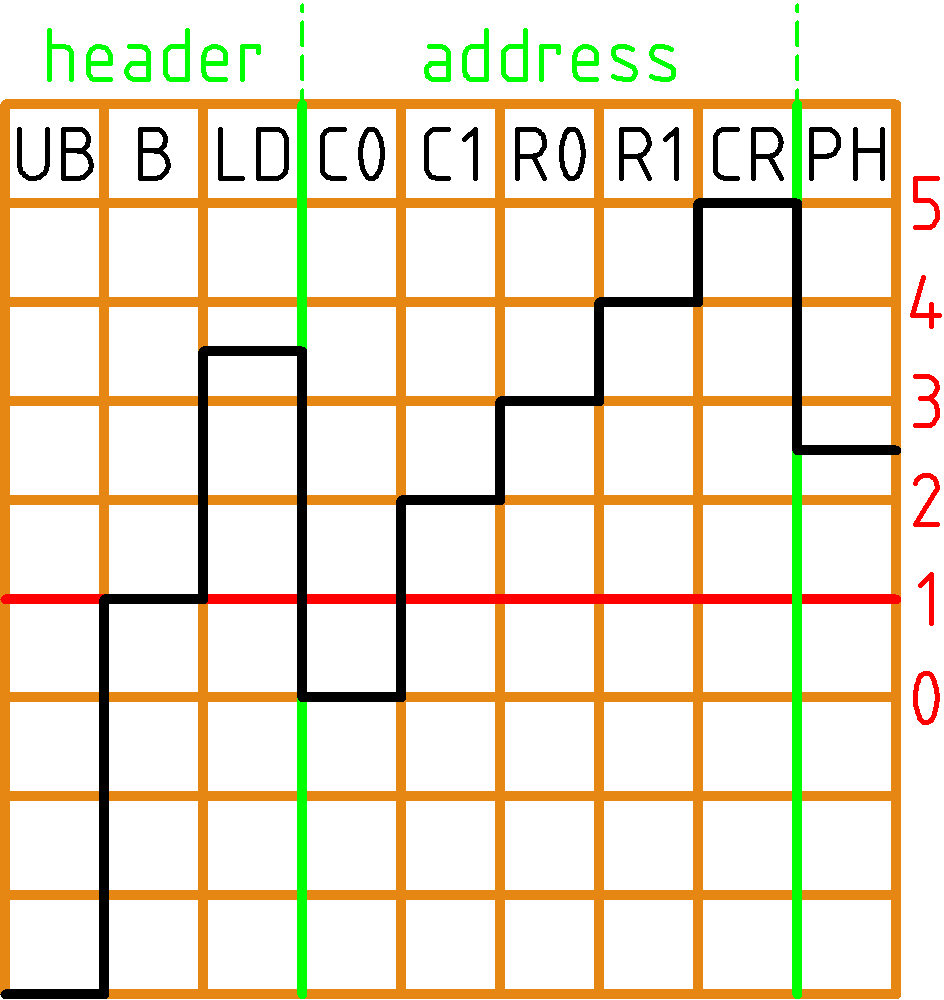
\includegraphics[width=0.47\textwidth]{levels}}
	\caption{Signals of the analogue \ac{ROC}}
	\label{procsig}
\end{figure}\no
% =======================
\subsubsection{\ac{I2C} Address}\label{si2c}
In order to be able to operate more than one \ac{ROC} with a single \ac{DTB}, every \ac{ROC} has a $4\,$bit \ac{I2C} address. The address can be set by connecting the supply pads $22-25$ to ground, of which each is equivalent to one bit. The bits are active if they are grounded, therefore the \ac{I2C} address is zero if none of the pads is connected. By sending commands to these addresses each \ac{ROC} can be programmed independently.
% =======================
\subsubsection{\ac{TBM}}\label{stbm}
\begin{figure}[ht]
	\centering
	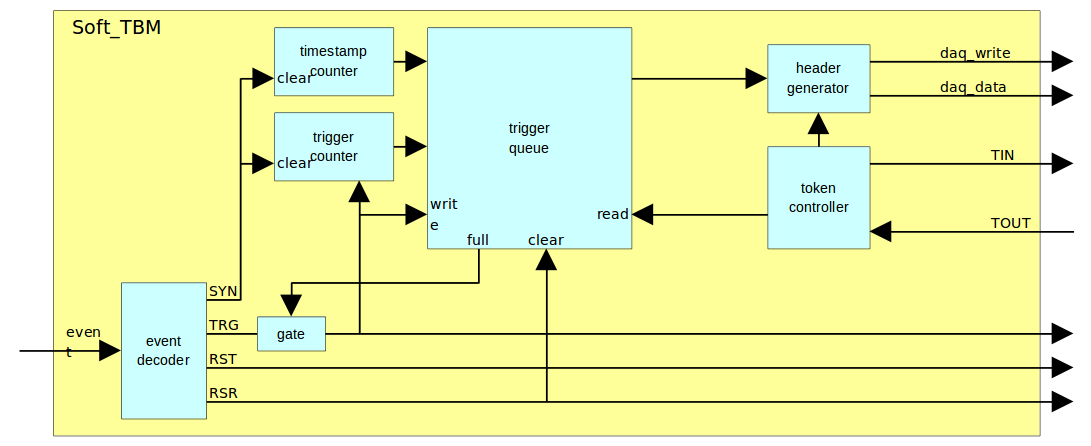
\includegraphics[width=0.95\textwidth]{tbm}
	\caption{Process chart of the emulated \ac{TBM}.}
	\label{ptbm}
\end{figure}\no
A process chart of the basic functionality of the \ac{DTB}'s \ac{TBM} is shown in \ar{ptbm}. While passing through the \ac{TBM} incoming triggers [TRG]  increment the $4./$bit trigger counter and write an entry into the trigger queue. This information is then read by the token controller, which sends out a token [TOUT] for each trigger and also receives the tokens [TIN] again that went to the \ac{ROC}. Once the token was received the the respective trigger gets cleared from the queue. The maximum amount of triggers in the trigger queue is $16$. If more triggers pile up until the [TIN] comes back, the triggers are caught by a gate where they are annihilated. There is also the possibility to clear the trigger queue with a reset signal. The token controller as well as the trigger queue send information to the header generator. When [TIN] arrives the header generator adds the information to the digital data stream in form of a header and a trailer, which each consist of two $16\,$ bit data words. The header contains an $8\,$bit event number and information about the trigger position inside the clock cycle.  The trailer contains, inter alia, a stack counter that is equivalent to the number of queued triggers. More information about the header and the trailer of the \ac{TBM} are given in \ar{stbmprob}. 
% ========================================================
\section{Digital Pixel Detector}\label{s23}
\begin{wrapfigure}{r}{4.5cm}
	\vspace*{-10pt}
	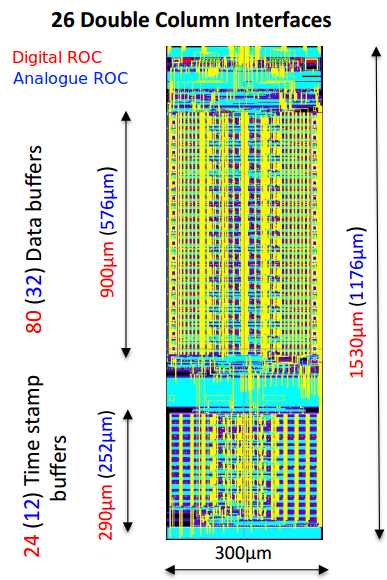
\includegraphics[width=4.4cm]{DigRocPeri}
	\caption{Double column interface of the digital \ac{ROC} \cite{hits}}
	\label{p12}
	\vspace*{-15pt}
\end{wrapfigure} 
For the Phase 1 Upgrade of \ac{CMS} a new digital \ac{ROC} was designed based on the analogue one. Their functionality is in principle still the same. An overview of the differences can be found in \ar{t3}.\\
One of the limitation of the analogue \ac{ROC} was a limited buffer size for the Level 1 trigger latency. To overcome this problem the number of data buffers was increased from $32$ to $80$. To reduce the readout related dead times due to higher rate, the number of time stamp buffers was doubled from $12$ to $24$. In addition the readout bandwidth had to be increased. This was done by switching to a fully digital readout by means of an on-chip \ac{ADC} for every \ac{DC}, new fast digital readout links, a \ac{PLL} to provide higher frequencies and some modifications to the control logic.An important feature of the new is the lower overall signal threshold that also increases the persistence of the chip \cite{hits}. This feature is indispensable for the low signals of diamonds, which is a possible candidate for a new generation of pixel chips. Going to lower thresholds was achieved by keeping the timewalk between the highest and lowest signal amplitudes within one clock cycle ($<16\,$ns) and reducing the cross talk in the digital \ac{ROC} layout as well as lower electronic noise. Besides, the output of the fast-Or signal was removed from the digital \ac{ROC}.\\
For easier usage the number of \ac{DAC} parameters is reduced to $16$. There is now only one parameter (\textit{vwllpr} and \textit{vwllsh}) for the pre-amplifier and the shaper instead of two and the leakage current compensation was removed. The six \ac{DAC}s for the double column periphery, which are responsible for the shape of the pulse height vs. \textit{vcal} curve, were condensed into \textit{vibias\_bus} and \textit{phoffset}. A comparison of the \ac{DAC}s that changed can be found in \ar{tdacchange}.
\begin{table}[ht]
	\centering
	\begin{tabularx}{0.85\textwidth}{X|l|l}\noalign{\hrule height 2pt}
			 &\multicolumn{1}{c}{\textbf{psi46v2}}	&\multicolumn{1}{|c}{\textbf{psi46dig}}	\\\hline
		\ac{ROC} size					& $7.9\times9.8\,$mm	& $7.9\times10.2\,$mm 	\\
		Pixel size						& $100\times150\,\upmu$m& $100\times150\,\upmu$m\\
		Smallest radius					& $4.3\,$cm				& $2.9\,$cm				\\
		\ac{DAC}s / registers			& $26$ / $3$			& $16$ / $3$			\\
		Power up condition				& not defined			& default values		\\
		Pixel charge readout			& analogue				& digitised, $8\,$bit	\\
		Readout speed					& $40\,$MHz				& $160\,$Mbit/s			\\
		Time stamp buffer size			& $12$					& $24$					\\
		Data buffer size				& $32$					& $80$					\\
		Output buffer FIFO				& no					& yes					\\
		Double column speed				& $20\,$MHz				& $40\,$MHz				\\
		Metal layers					& $5$					& $6$					\\
		leakage current compensation	& yes					& no					\\
		In-time threshold				& $3500\,$e				& $<2000\,$e			\\
		\ac{PLL}						& no					& yes					\\
		Data loss at max 				& $\sim3.8\,$\% at  	& $\sim3\,$\% at		\\
		operating flux					& $120\,$Mhz/cm$^{2}$	& $580\,$Mhz/cm$^{2}$ \footnotemark[2]\\\noalign{\hrule height 2pt}
	\end{tabularx}					
	\caption{comparison between analogue and digital \ac{ROC} \cite{hits}}
	\label{t3}
\end{table}\no
\footnotetext[2]{This is valid for the layer 1 version of the digital chip, that is planned for the Phase 1 Upgrade.}
\begin{table}[ht]
	\begin{tabularx}{\textwidth}{c|l|l|X}
		\noalign{\hrule height 2pt}
		\textbf{\#} & \multicolumn{1}{l}{\textbf{analogue}} & \multicolumn{1}{|l}{\textbf{digital}}	& \multicolumn{1}{|l}{\textbf{comment}}\\\noalign{\hrule height 2pt}
		\multicolumn{4}{c}{\textbf{Analogue Signal (\ac{PUC})}}							\\\hline
		$05$ &	vleak				& $-$ 		& leakage current compensation removed			\\
		$06$ &	vrgpr				& $-$ 		& combined into vwllpr		\\	
		$07$ &	vwllpr				& vwllpr	&							\\
		$08$ &	vrgsh				& $-$		& combined into vwllsh		\\
		$09$ &	vwllsh				& vwllsh	&							\\\noalign{\hrule height 2pt}
		\multicolumn{4}{c}{\textbf{Double Column Periphery}}				\\\hline
		$13$ &	vibias\_bus 		& vibias\_bus	&						\\
		$14$ &	vbias\_sf			& $-$			&						\\
		$15$ &	voffsetop			& $-$			& the six periphery dacs\\
		$16$ &	vibiasop			& $-$			& were condensed into two \\
		$17$ &	voffsetroc			& phoffset		& 						\\
		$18$ &	vion				& $-$			&						\\\noalign{\hrule height 2pt}
		\multicolumn{4}{c}{\textbf{Control and Interface Block}}			\\\hline
		$19$ &	vibias\_dac 		& vcomp\_adc 	&						\\
		$20$ &	vibias\_ph 			& phscale 		& 						\\
		$21$ &	vibias\_roc 		& $-$			& removed				\\\noalign{\hrule height 2pt}
		\multicolumn{4}{c}{\textbf{Fast-OR Trigger (\ac{PUC})}}				\\\hline
		$22$ &	vicolor 			& vicolor	&							\\
		$23$ &	vnpix 				& $-$		& fast-OR removed			\\
		$24$ &	vsumcol	 			& $-$		& fast-OR removed			\\
		\noalign{\hrule height 2pt}
	\end{tabularx}					
	\caption{Different \ac{DAC}s for analogue and digital \ac{ROC}}
	\label{tdacchange}
\end{table}\no
% ========================================================
\section{Digital Test Board}\label{sdtb}
The psi46 \ac{DTB} is the interconnect between a computer and the \ac{ROC}. In the past the analogue chips were operated with an \ac{ATB}, which has some major disadvantages in comparison with the \ac{DTB}. For example it has only a limited amount of data it can save, s.t. during beam tests one could only take runs of $300000$ events until the buffer was full. One of the achievements of this thesis is the possibility to reliably operate analogue chips as well as digital chips with the \ac{DTB}.\\
The \ac{DTB} is powered by a $6\,$V AC to DC power supply and connects via an adapter to the \ac{ROC}. It has two interfaces to a computer of which the ethernet is not implemented yet, leaving the USB 2.0 as only option. In here lies another advantage compared to the \ac{ATB}, which only had a USB 1.1 connection: The writing speed is increased a lot. In order to use several \ac{DTB}s on the same computer, each \ac{DTB} has its own serial number. Once connected to the chip and a computer, the \ac{DTB} and its \ac{FPGA} are completely controlled with a software called pXar. The \ac{FPGA}, which is emulating the \ac{TBM}, has its own firmware developed at \ac{PSI}. By now there more than twenty iterations of this firmware, which can be easily upgraded via USB. During this thesis the firmware versions from $4.0$ to $4.2$ were utilised.\\
It is possible to read out several signals of the \ac{DTB}. For that purpose there are two digital and two differential analogue LEMO outputs.\\
Furthermore the \ac{DTB} has inputs for an external clock and trigger, which accept \ac{TTL} signals. The height of the external trigger signal has to be at least $3\,$V to guarantee stability. Since these inputs are not terminated, it is very important to terminate incoming signals at the input to avoid reflections inside the cables. The \ac{DTB} also has a \ac{HV} input that is able to distribute the \ac{HV} to the sensor.
\begin{figure}[ht]
	\centering
	\subbottom[Top view.]{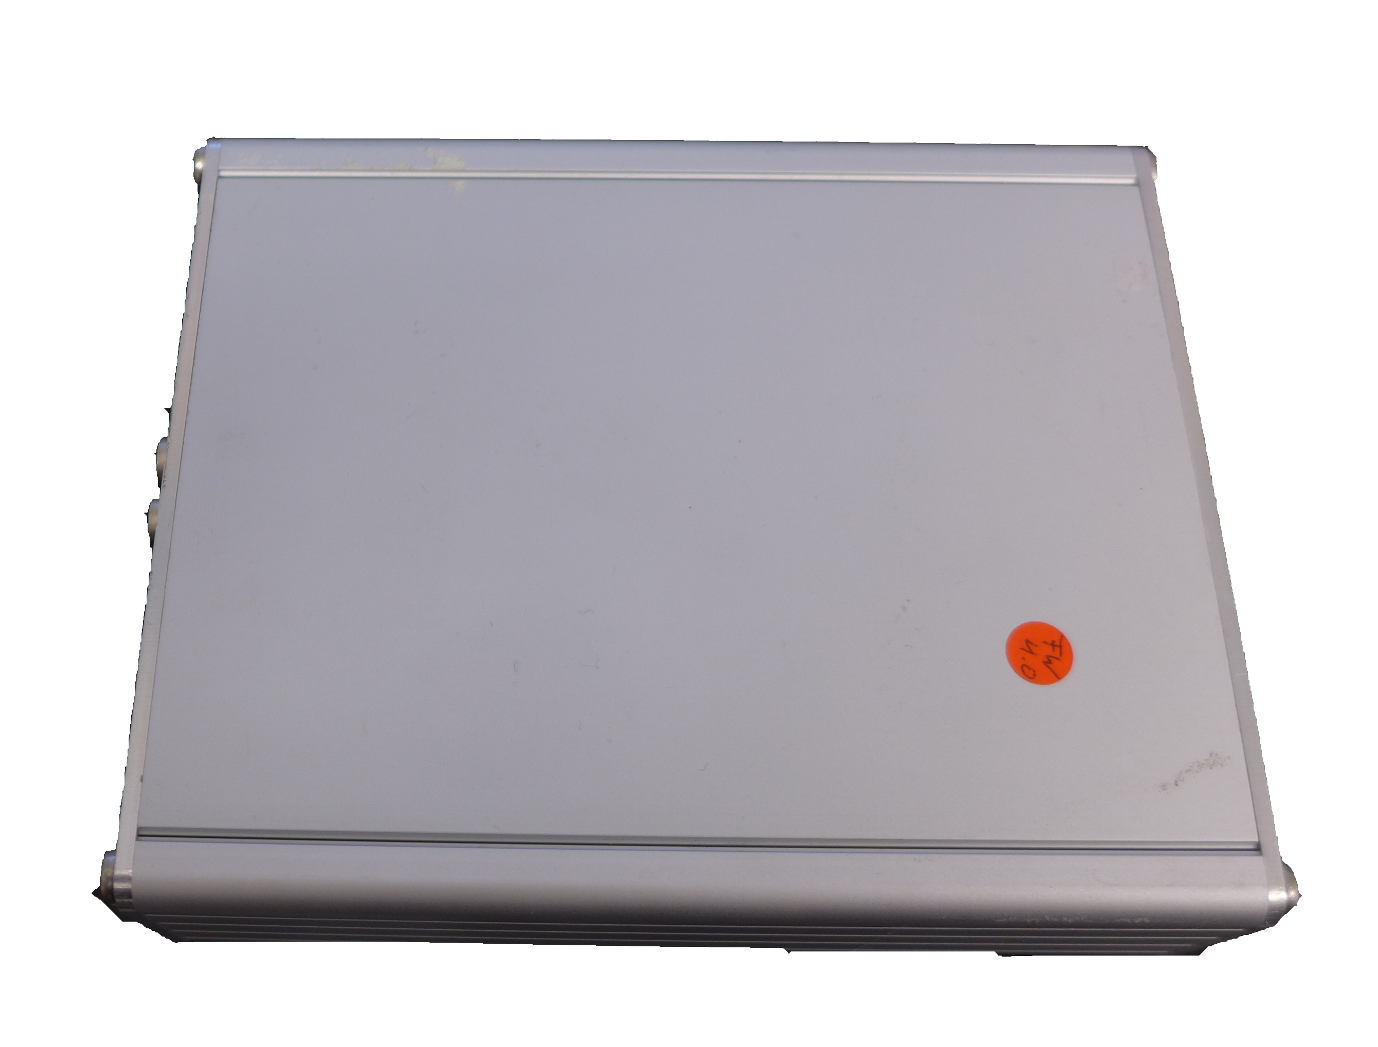
\includegraphics[width=0.47\textwidth]{DTB}\label{p10}}
	\hfill
	\subbottom[Front and backside.]{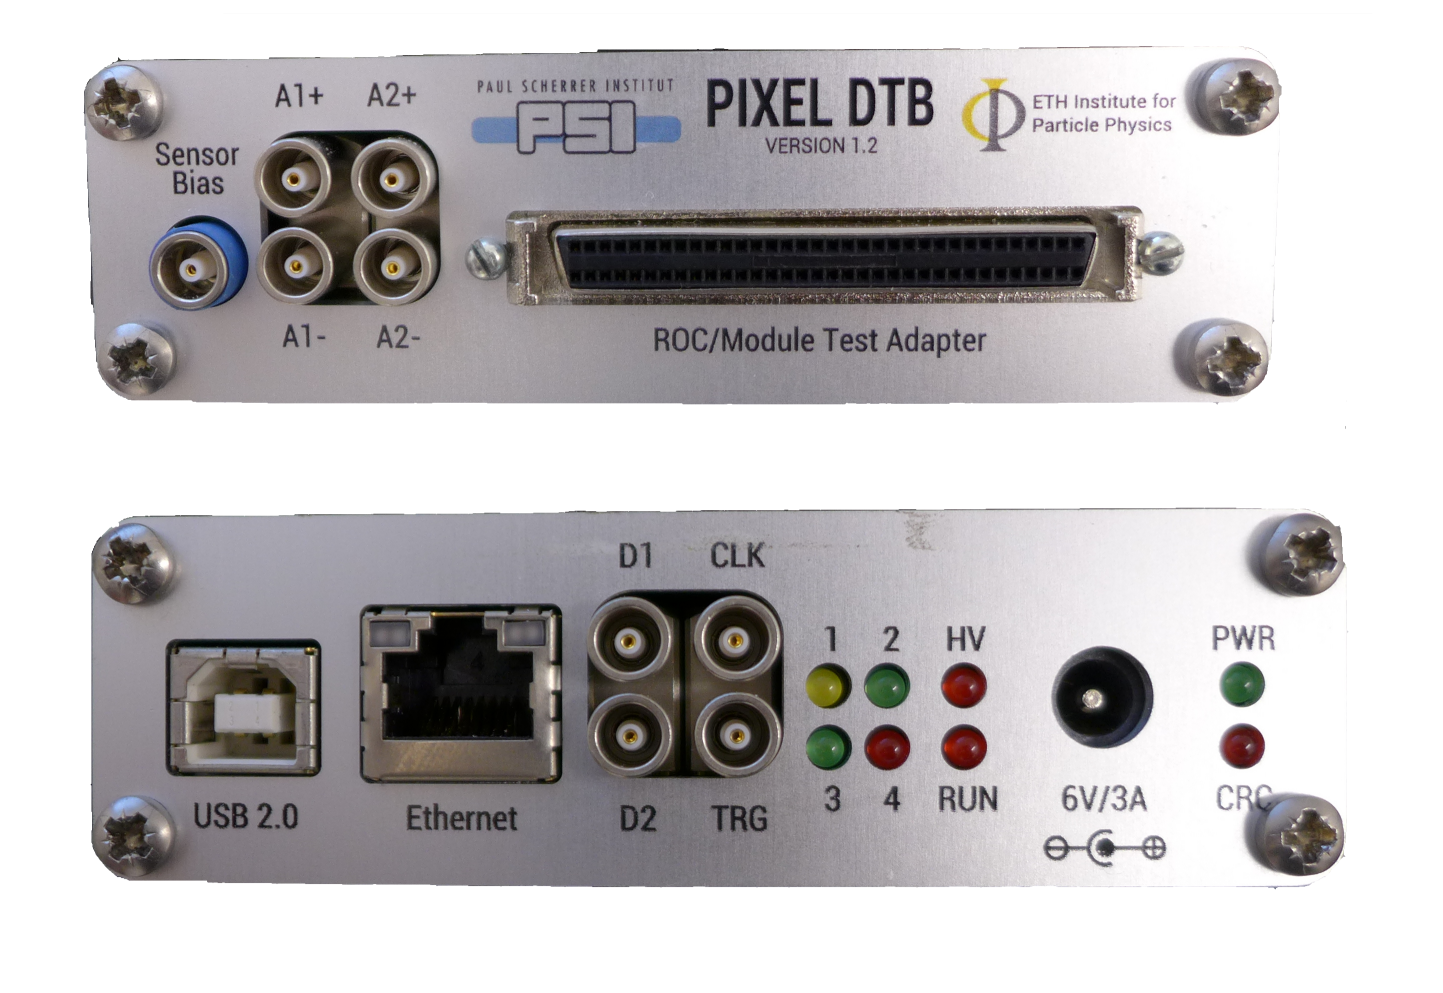
\includegraphics[width=0.47\textwidth]{DTB-Sides}\label{p11}}
	\caption{Photographs of the \ac{DTB}.}
	\label{pdtb}
\end{figure}\no
% ========================================================

\chapter{The Material Behind the Curtain - Theory}
\chapter{The Foundation of the Experiment - Telescope}
% ========================================================
% INTRO
% ========================================================
\section{Introduction}\label{s20}
The Compact Pixel Tracking Telescope has two different versions that were both constructed at \ac{ETH} in Z{\"u}rich. It is called telescope due to the fact that it utilises different single planes to get information about a \ac{DUT}. Its main purpose is to provide an event trigger and high resolution tracks.\\ 
To accomplish that goal it consists of several single \ac{CMS}-Pixel chips that are placed consecutively, perpendiclar to the beam. The chips are mounted on so-called adapter planes and have a fixed distance to one another that is given by the connectors of the connectors of the motherboard.\\
The planes are daisy chained and are read out by the \ac{DTB} which makes them accessible via a computer.
% ========================================================
% 1
% ========================================================
\section{Telescope Layout}\label{s21}
As already mentioned above, there are two versions of the telescope. Version 1 was designed to be as simple as possible and consists of six planes with analogue chips. Whereas the second version that was built on the experience with first one, comprises three plane modules, which may be combined to bigger modules. The modules of version 2 can consist either of digital chips or of analogue chips. Version 2 has some additional features as well that will be mentioned in the following.\\
Both consist mainly of three parts: a motherboard, adapter planes and the \ac{ROC}s.
% ========================================================
\subsection{Motherboard}\label{s210}
The motherboard is the main frame of the telescope. Pictures of the motherboards are shown in \ar{pmb}, the number in square bracket in the following text refer to the numbers in the pictures.\par
\begin{figure}[h]
	\centering
	\subbottom[Version 1]{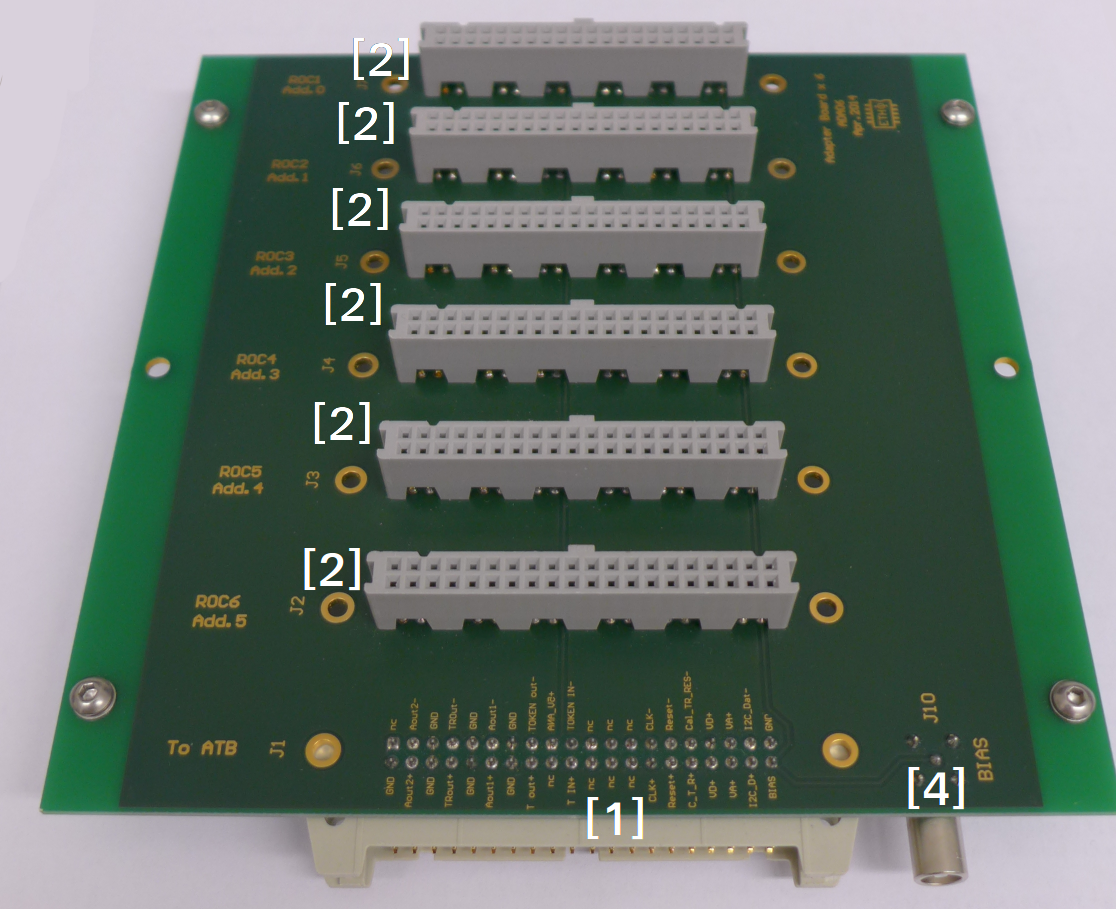
\includegraphics[width=0.52\textwidth]{setup/mb1}\label{p0}}
	\hfill
	\subbottom[Version 2]{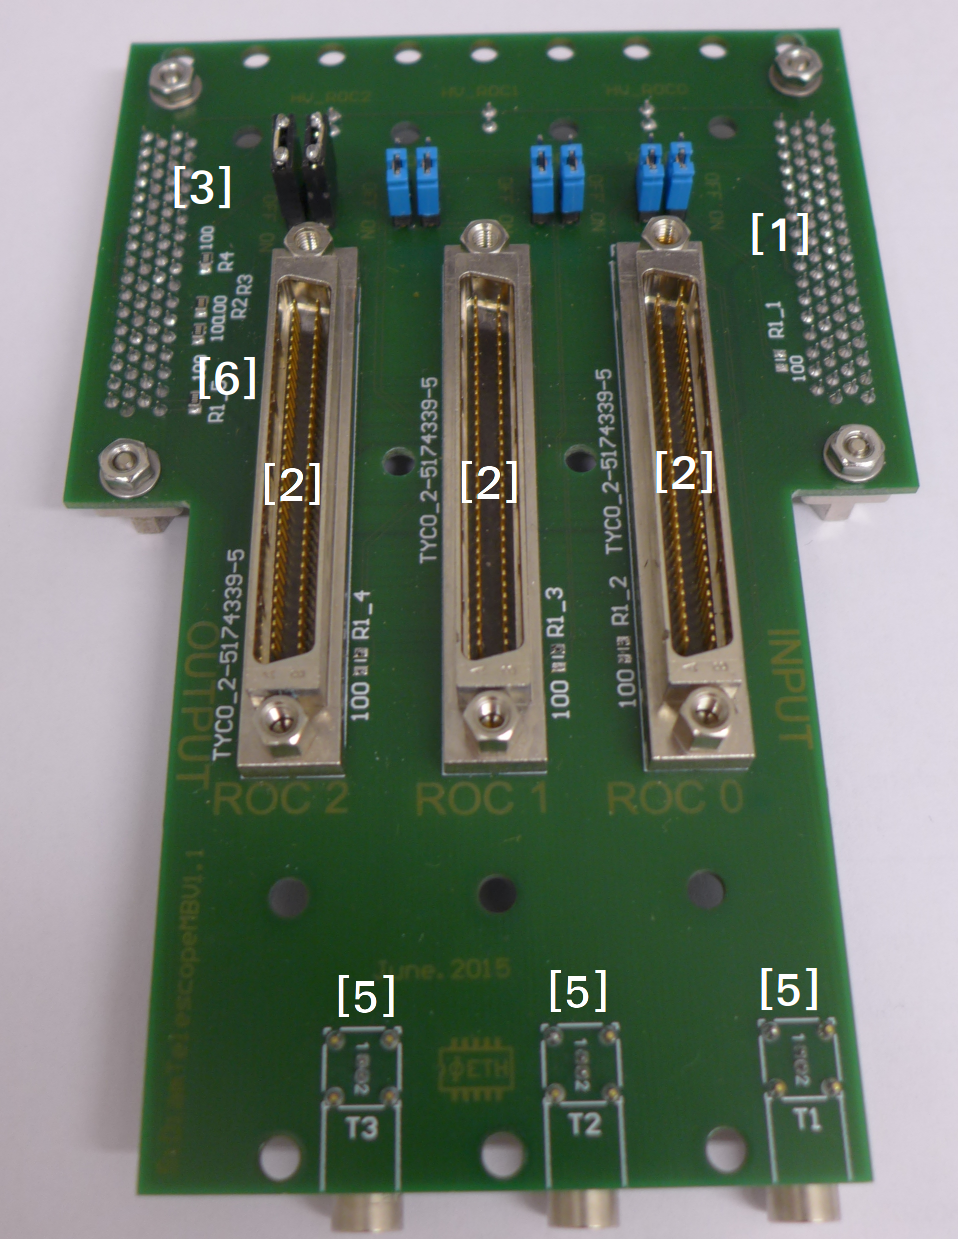
\includegraphics[width=0.42\textwidth]{setup/mb2}\label{p1}}
	\caption{The motherboards of the two telescopes}
	\label{pmb}
\end{figure}\no
The \ac{PCB} has a male connector [1] for a data transfer cable to communicate with a test board. In case of version 2 there is a second male [3] connector to which another telescope may be connected and that can only be used only as an output of the data stream. Next in line after the input come several daisy chained female connectors [2] to plug in the adapter planes. In order that the token can be sent through the whole chain, either the planes have to be plugged into [2] or a token jumper (\ar{pjumper}) has to be used. In addition version 1 has a LEMO connector [4] that allows to bias all of the connected sensors and version 2 has a differential LEMO outputs [5] for the fast-OR of every plane. All signals that pass through the telescope are properly terminated by resistors on the motherboard\footnote{In case of version 1 the resistors are underneath the board}. In case of version 2 there are boards with and without resistors and one should take care that only the last board in the chain is one with termination. Otherwise the signals might get too low to be measured.\\
The main differences of the two versions are stated in \ar{t1}.\\
The version 1 of the telescope was limited to a maximum of six static analogue planes. A main advantage of the other version is its flexibility to chain multiple three-plane telescopes together. Furthermore it easier and more convenient to place the token jumpers now. The Dimensions of the two telescopes are shown in \ar{pdim}.
\begin{table}[ht]
	\begin{tabularx}{\textwidth}{X|c|c}
		\noalign{\hrule height 2pt}
										& Version 1 			& Version 2 					\\\hline
		Connector type 					& ATA 40 pin 			& VHDCI 68 pin					\\			
		Number of planes per telescope 	& $6$ 					& $3$							\\
		Maximum number of Planes per read out chain		& $6$					& $3\times3$ \footnotemark[2] \\
		Fast-OR	output					& directly on the plane	& on the motherboard			\\
		Token jumper					& \ar{pjumper1}				& \ar{pjumper2}	\\
		\noalign{\hrule height 2pt}
	\end{tabularx}					
	\caption{Differences between the two motherboard versions}
	\label{t1}
\end{table}\no
\footnotetext[2]{Theoretically one could chain an infinite amount of telescopes. In reality the timing between the planes gets worse the longer the data has to travel, s.t. it not possible to read out more than three connected telescopes.}
\begin{figure}[ht]
	\centering
	\subbottom[Version 1: Self crafted token jumper by hard wiring the token line of a spare ATA connector. This jumper is then placed on the connector of the motherboard instead of a plane.]{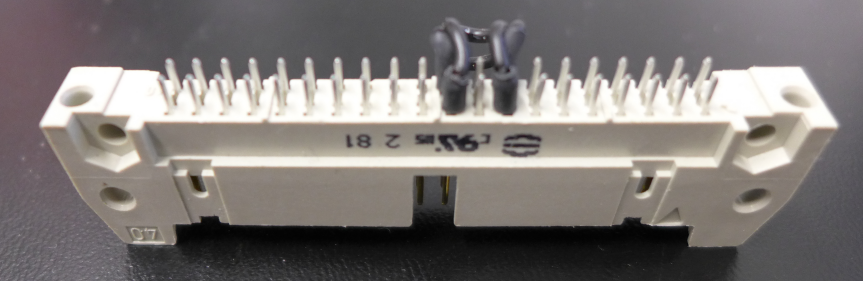
\includegraphics[width=0.47\textwidth]{TokenJumper}\label{pjumper1}}
	\hfill
	\subbottom[Version 2: The blue jumpers loop the token into the plane and the black jumpers make the token pass the plane. A blue jumper at the ``Out'' position will send the token into the next connected motherboard and a black one back to the \ac{DTB}]{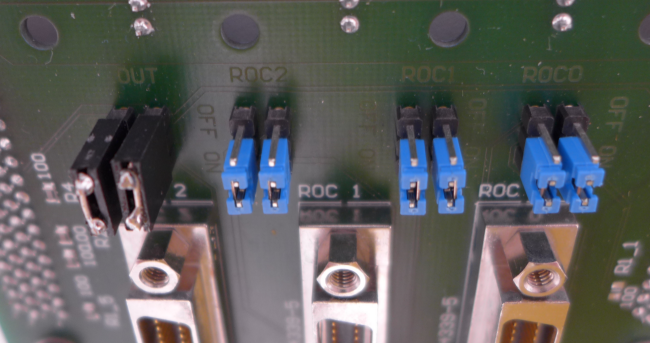
\includegraphics[width=0.47\textwidth]{setup/jumper2}\label{pjumper2}}
	\caption{The token jumpers for the two version of the telescope.}
	\label{pjumper}
\end{figure}\no
\begin{figure}[ht]
	\centering
	\subbottom[Version 1]{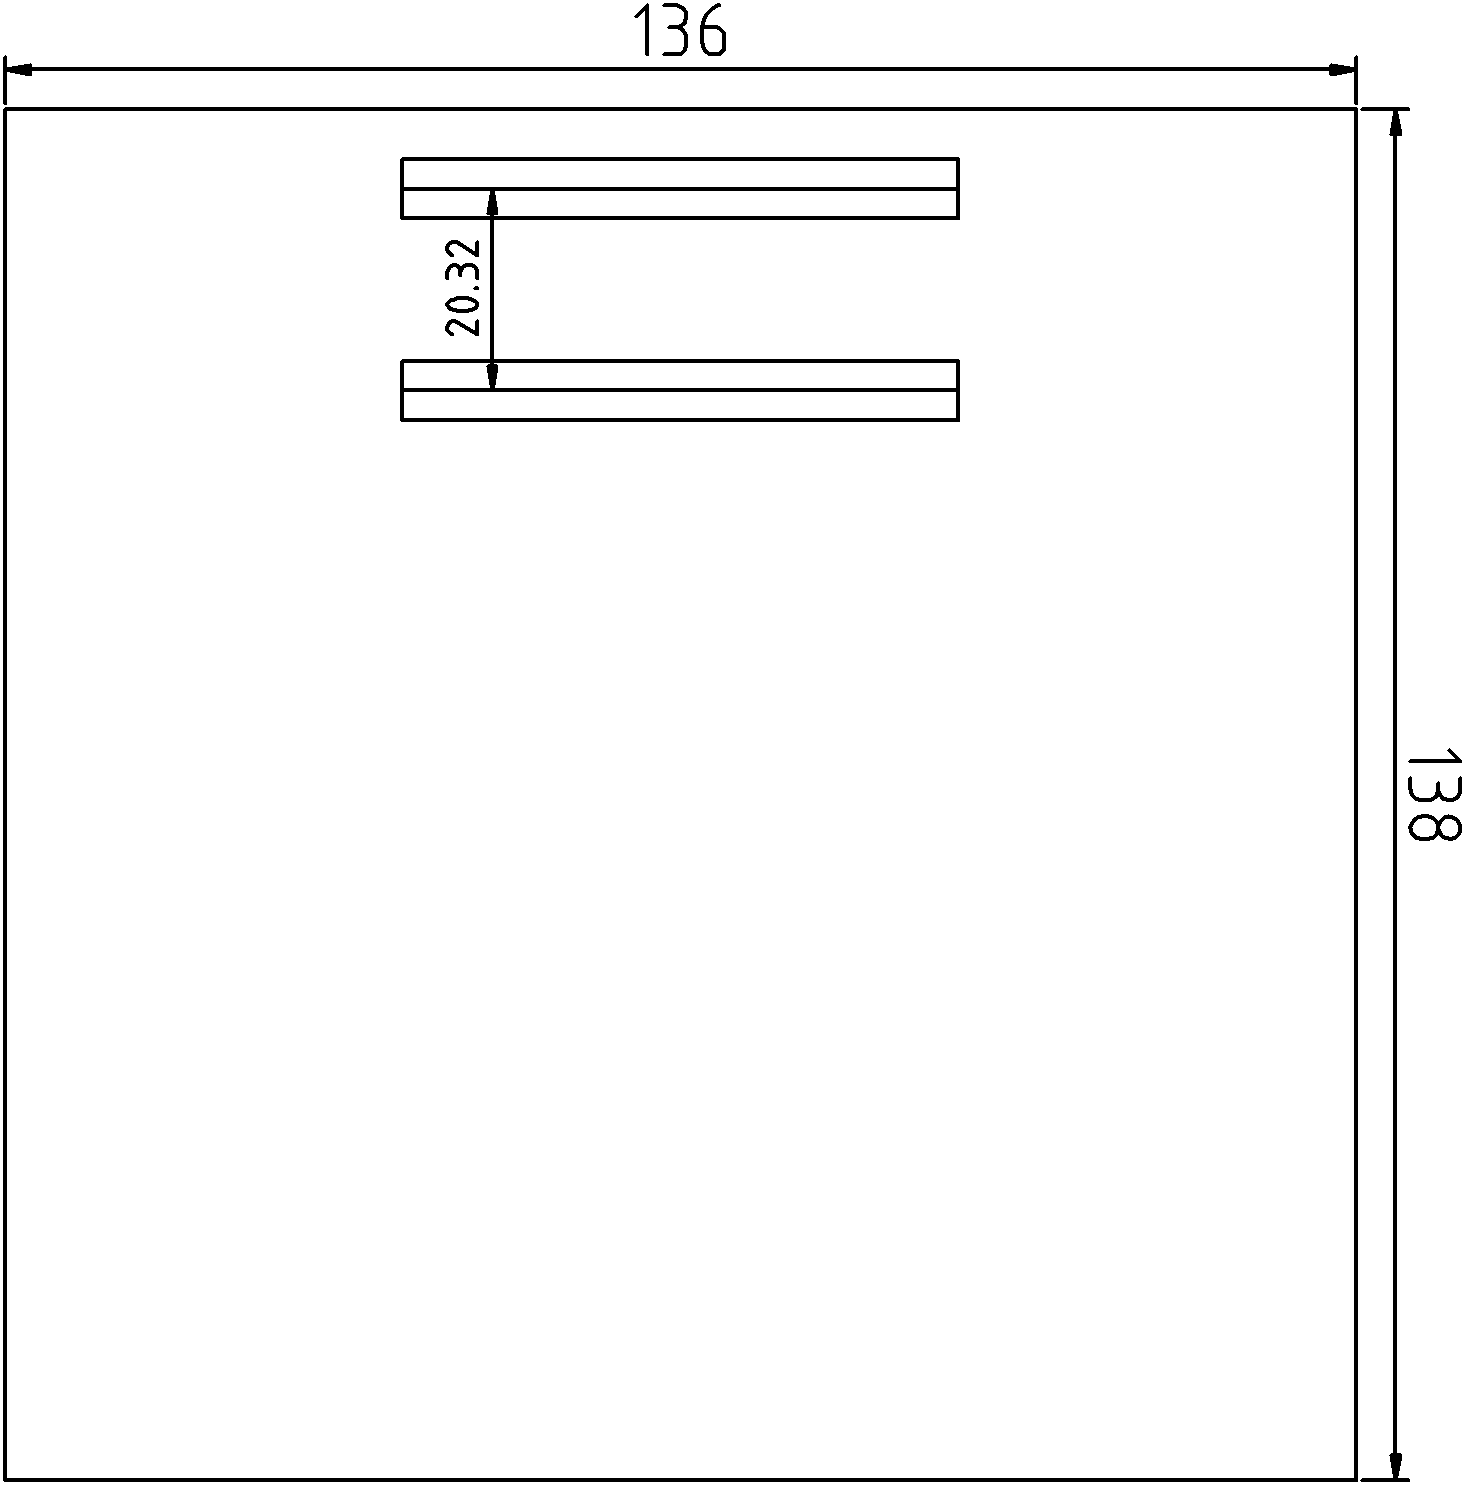
\includegraphics[width=0.47\textwidth]{dim1}\label{pdim1}}
	\hfill
	\subbottom[Version 2]{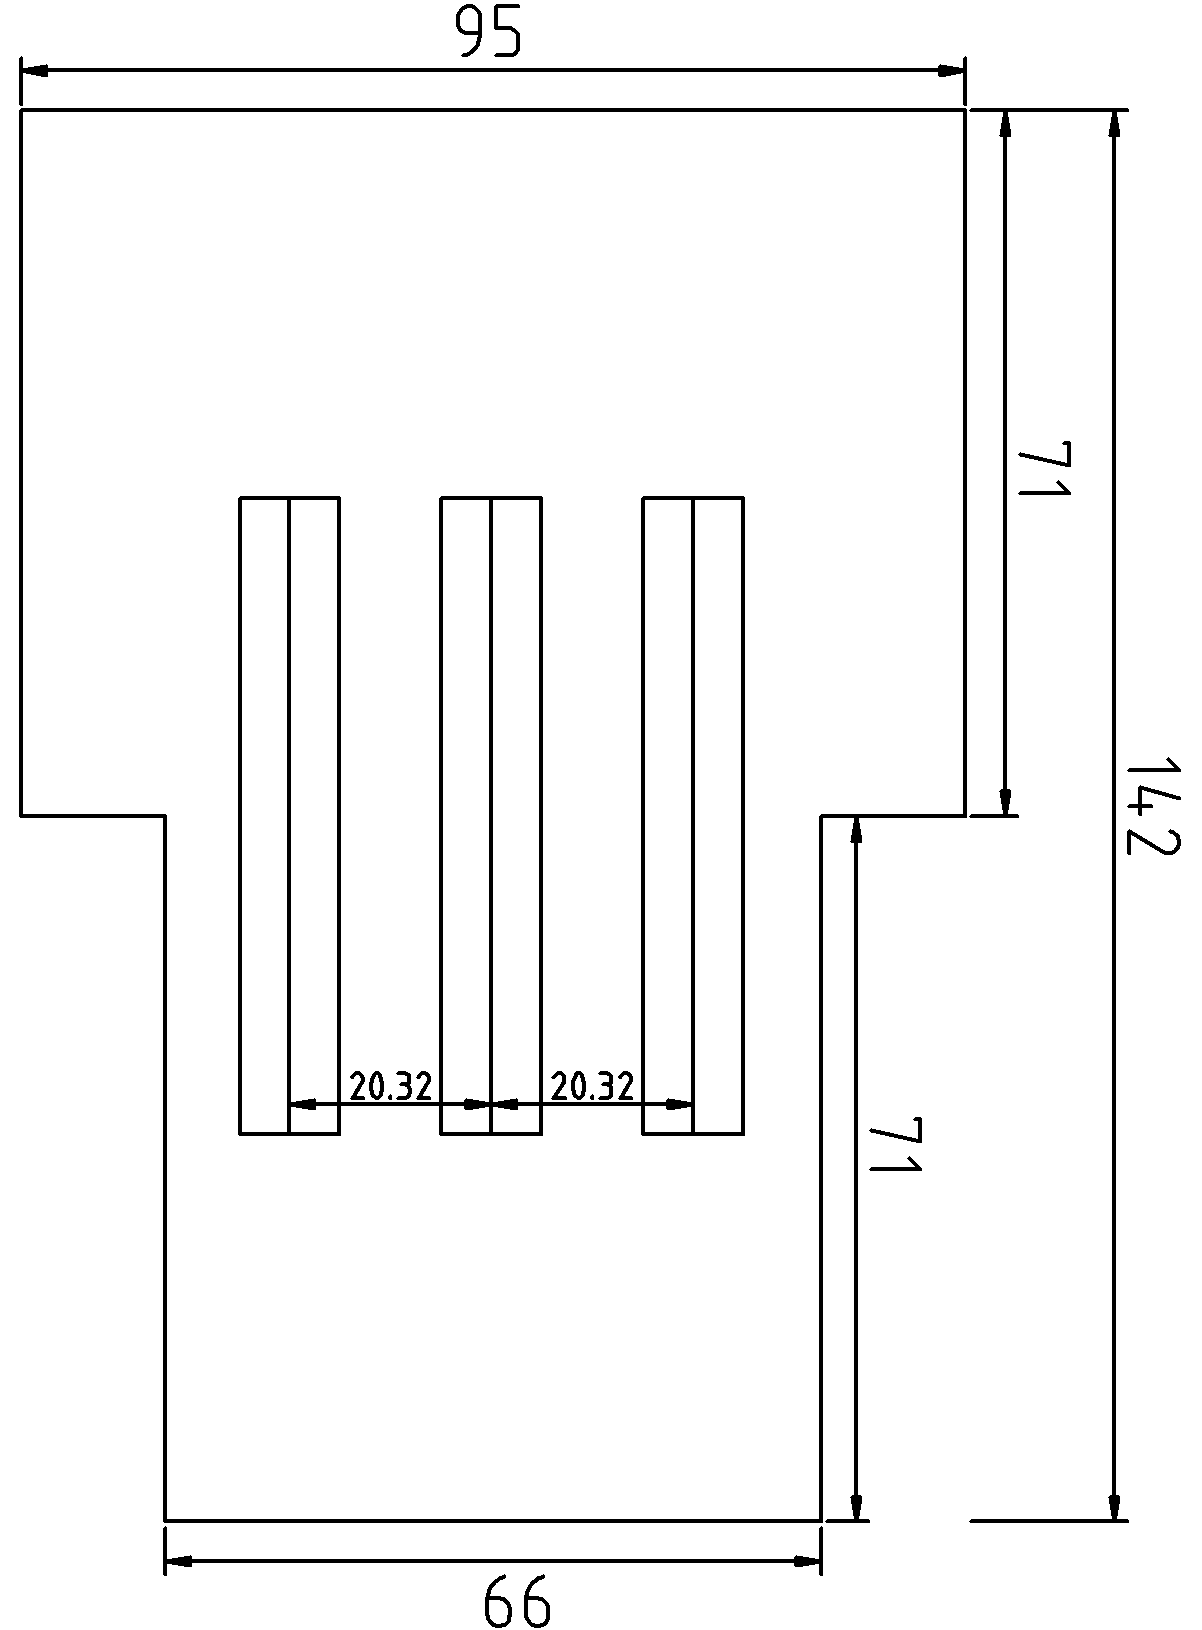
\includegraphics[width=0.47\textwidth]{dim2}\label{pdim2}}
	\caption{Dimensions of the two motherboards in millimetres.}
	\label{pdim}
\end{figure}\no
% ========================================================
\newpage
\subsection{Adapter Plane}\label{s211}
The adapter plane is the link between the telescope and a single \ac{CMS}-Pixel 
\begin{wrapfigure}{r}{5cm}
	\vspace*{-10pt}
	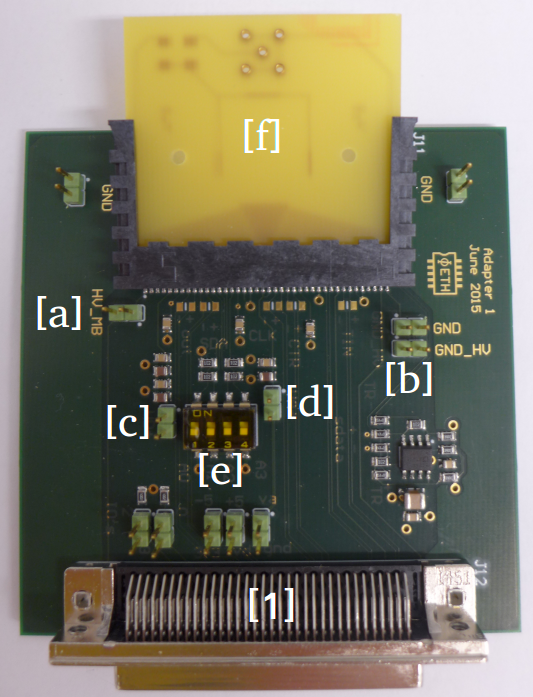
\includegraphics[width=5cm]{setup/digada}
	\caption{Digital adapter plane.}
	\label{p6}
	\vspace*{-5pt}
\end{wrapfigure} 
chip. The numbers in the following description refer to parts in \ar{p6} and \ar{padaana}. On the bottom end of the \ac{PCB} is a male connector [1] with which the plane can be plugged directly into the motherboard. The analogue planes of both telescope versions are very similar. Their differences are the already mentioned type of connector (\ar{t1}) and that there are two differential outputs for the fast-OR on the PCB of version 1 [2] (\ar{p4}) that were moved to the motherboard in version 2. Apart from that they both have an input for biasing the sensor [3], an amplifying circuit for the fast-OR [4], a small cable connector [5] to the \ac{ROC}\footnote[3]{This connector was already used for the \ac{PLT} and was kept since then.} and cable pins [6] to bias the \ac{ROC}. In version 2 there is an additional jumper [7] to allow biasing from either the adapter plane or via the connector to the motherboard. In both cases, the BIAS-GND pin of [8] has to be connected to the other outer pin of [8]. In order to bias the \ac{ROC} a cable [9] has to be connected from the BIAS- pin of [6] to the \ac{ROC} itself.\\
The adapter for the digital chips, which is shown in \ar{p6}, can only be used in combination with version 2 and differs a bit from the analogue one. The only way to bias the digital chips is via the test board and the SCSI connector, which means that there has to be a jumper at HV-MB [a] and GND-HV [b]. Likewise two jumpers have to connect the supply voltages VD [c] and VA [d] to the chip. Another very useful improvement is the dip switch box [e] in the middle of the plane, which allows to set any \ac{I2C} address between $0$ and $15$. Since the digital chips are put on special \ac{PCB}s [f], the adapter has a completely different mounting system, s.t. the chips can be easily plugged in and out, whereas the analogue \ac{ROC}s have to be screwed to the \ac{PCB}.
\begin{figure}[ht]
	\centering
	\subbottom[Version 1 without \ac{ROC}]{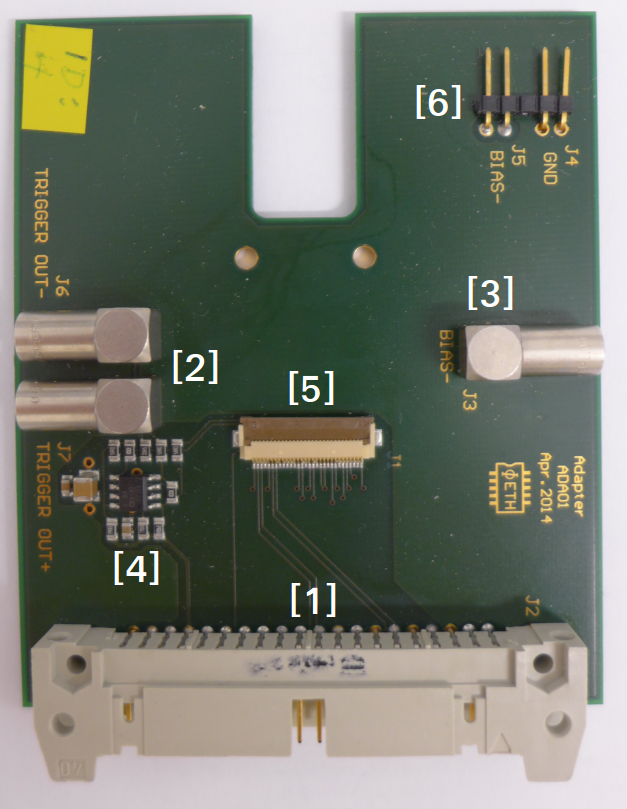
\includegraphics[width=0.47\textwidth]{setup/adaana1}\label{p4}}
	\hfill
	\subbottom[Version 2 with \ac{ROC} mounted underneath the black cover]{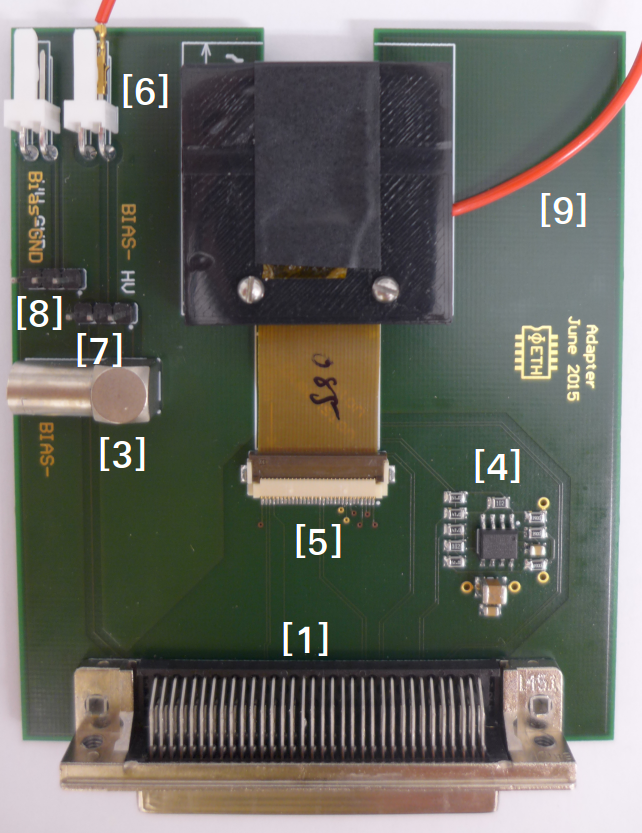
\includegraphics[width=0.47\textwidth]{setup/adaana2}\label{p5}}
	\caption{Analogue adapter planes of the two telescope versions.}
	\label{padaana}
\end{figure}\no
% ========================================================

\chapter{The Order of Matter - Set-up}
\chapter{The Doorway to the Information - Data Acquisition}

% ========================================================
% INTRO
% ========================================================
\section{Introduction}
In this chapter I am going to explain how the interfacing between a computer and the telescope is working, in which way the \ac{ROC} can be programmed and how the data is acquired and decoded by the software.\\
Basically all communication between the telescope and a computer is done via program called pXar, short for Pixel eXpert Analysis Readout, a pixel chip \ac{DAQ} and test suite. It was written by Simon Spannagel and Urs Langenegger to operate the digital \ac{ROC}. The program is completely composed in C++ and the main part, which talks to and programs the chips via the \ac{DTB}, is confined the so-called pXar-core and consists of a \ac{HAL} and an \ac{API}. Using the basic functions from the pXar-core library there are already a variety of tests that can be performed via the pXar-\ac{GUI}. For easier access and better flexibility Simon Spannagel also wrote a cython translation of the main pXar-core functions to make them accessible via python, which has the huge advantage to easily write own tests and use them via a python \ac{CLI}. To save the data of a single telescope one could also use pXar software, but since we are interested in the data combining with other instruments, e.g. pad detectors or second telescope, it is much more convenient to use the EUDAQ software.
% ========================================================
%TODO PUT that in the appendix
\section{Software}
The master branch of pXar and my own branch can be downloaded from git: 
\begin{itemize}
	\item \url{https://github.com/psi46/pxar}
	\item \url{https://github.com/michareichmann/pxar}
\end{itemize}
More information as well a detailed installation instruction can be found at the \ac{CMS} twiki: 
\begin{itemize}
	\item \url{https://twiki.cern.ch/twiki/bin/viewauth/CMS/Pxar} $rightarrow$ branch eth-2.0
\end{itemize}
The version of EUDAQ we were using can be found here: 
\begin{itemize}
	\item \url{https://github.com/veloxid/eudaq-drs4}. 
\end{itemize}
% ========================================================
% 1
% ========================================================
\section{pXar Core}

\includegraphics[width=4cm]{pxar_logo}
includes more than the main functions of the pXar-core I am going to present, but these are the components everything else is built on and I was using most of the time. An overview of the full software architecture is shown in \ar{p13}, the core consists of \ac{HAL} and \ac{API}.\\
The NIOS II soft core \ac{CPU} is a synthetic \ac{CPU} that is embedded in the \ac{FPGA} of the \ac{DTB}. It runs at $50\,$MHz and is used to perform very simple commands like starting the pattern generator. It's main purpose is the control of the \ac{DTB} functionality. Since the correct commands are automatically picked by the \ac{API} of the pXar-core, it is not further investigated. For further information look at \cite{spannagel}.
\begin{figure}[ht]
	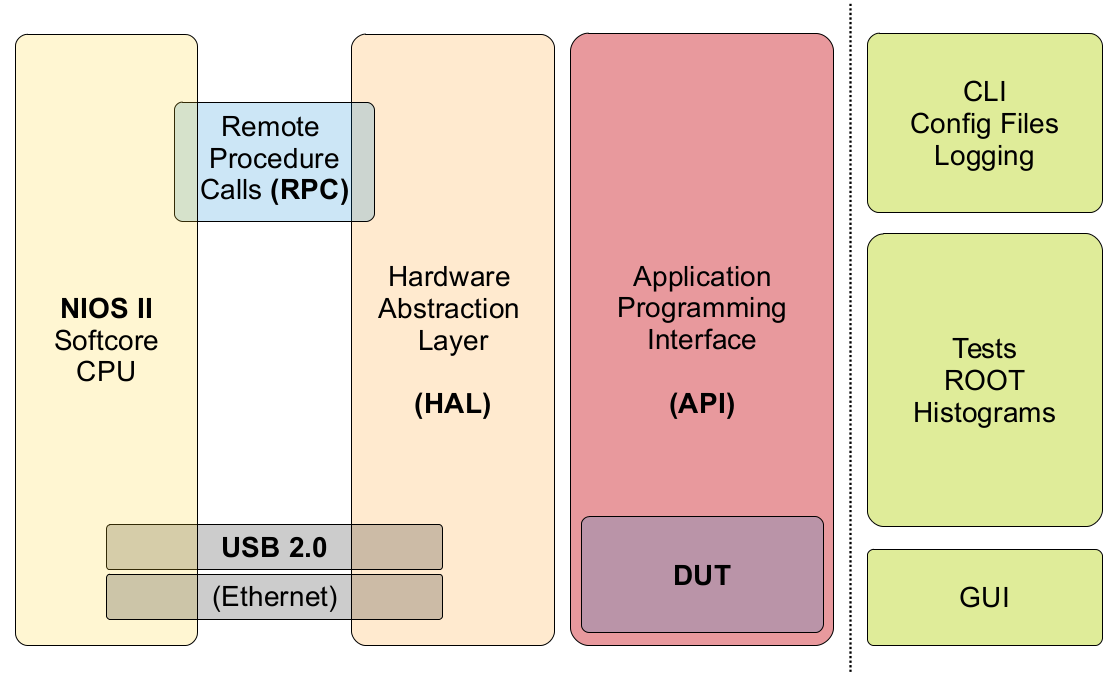
\includegraphics[width=0.95\textwidth]{pxar_scheme}
	\caption{software architecture of pXar \cite{spannagel}}
	\label{p13}
\end{figure}
% ========================================================
\subsection{\ac{HAL}}
The \ac{HAL} of the pXar-core is responsible for the direct communication with the \ac{DTB}. This is the part that has access to the RPC and USB. It supervises the data readout using pipes, which is a buffered readout of the data from the test board.\\
\hspace*{\dimexpr0.5\linewidth-5cm}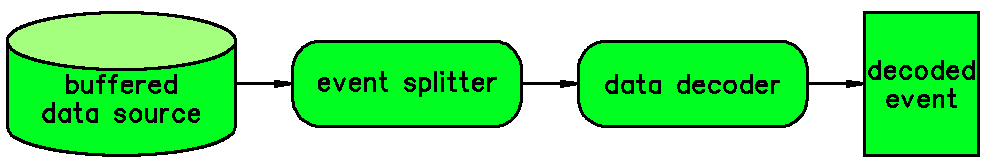
\includegraphics[width=10cm]{hal_buf}\\
The pipes can be set up for different purposes, either to deliver fully decoded events or ``raw'' events that are only split by the emulated \ac{TBM} header and trailer or complete raw data from the \ac{DTB}. The second option is very useful to debug the system, because it makes it easier to decide why something is not working. The last option may be useful for debugging too, but is mainly used for saving the raw data to a binary file.\\
Most of the basic functions with a short explanation are listed in \ar{t5}. They are loosely divided in categories i.e. basically all them can be used while the \ac{DTB} and pXar are running. So, having them in the group ``Device Initialisation'', means that they are used while initialising the board even though the may be reused afterwards.  \\
\begin{table}[ht]
	\begin{tabularx}{\textwidth}{l|X}
		\noalign{\hrule height 2pt}
		\multicolumn{2}{c}{\textbf{Device Initialisation}}							\\\noalign{\hrule height 2pt}
		\multicolumn{1}{c}{\textbf{command}}	& 	\multicolumn{1}{c}{\textbf{purpose}}	\\\hline
		initTestboard		& initialises the \ac{DTB} with its device specific \textit{signal delay} settings		\\
		setTestboardPower	& sets the \textit{analogue} and \textit{digital voltage} and \textit{current limits}		\\
		setTestboardDelays	& sets \textit{signal delay} settings		\\
		flashTestboard		& flashes a given \textit{firmware file} to the \ac{FPGA}		\\
		initROC				& initialises a \ac{ROC}s of a given \textit{type} with \textit{\ac{I2C} address} with a \textit{vector of \ac{DAC}s} 		\\
		SetupPatternGenerator	& sets the \ac{PG} to a given sequence		\\
		SetClockSource		& set clock source to internal or external		\\
		\noalign{\hrule height 2pt}
	\end{tabularx}
	\caption{base commands of \ac{HAL}}
	\label{t5}
\end{table}

\begin{table}[ht]
	\begin{tabularx}{\textwidth}{l|X}
		\noalign{\hrule height 2pt}
		\multicolumn{2}{c}{\textbf{\ac{DTB} Commands}}							\\\noalign{\hrule height 2pt}
		\multicolumn{1}{c}{\textbf{command}}	& 	\multicolumn{1}{c}{\textbf{purpose}}	\\\hline
		getTBia			& reads analogue current from \ac{DTB}		\\
		getTBva			& reads analogue voltage		\\
		getTBid			& reads digital current		\\
		getTBvd			& reads digital voltage		\\
		set*			& sets the limit of *$=$TBia, TBva, TBid, TBvd		\\
		SignalProbe*	& lays one of the internal \textit{signals} to the output *$=$D1, D2, A1, A2 		\\
		HVoff			& disables the \ac{HV} from the \ac{DTB} to the \ac{ROC}		\\
		HVon			& enables \ac{HV}		\\
		Pon 			& turns on power of the \ac{DTB}		\\
		Poff			& turns off power		\\
		rocSetDAC		& sets the \textit{\ac{DAC}} with \textit{\ac{I2C}} to a given \textit{value} 		\\
		\noalign{\hrule height 2pt}
	\end{tabularx}
	\caption{base commands of \ac{HAL}}
	\label{t6}
\end{table}

\begin{table}[ht]
	\begin{tabularx}{\textwidth}{l|X}
		\noalign{\hrule height 2pt}
		\multicolumn{2}{c}{\textbf{\ac{DAQ} Functions}}							\\\noalign{\hrule height 2pt}
		\multicolumn{1}{c}{\textbf{command}}	& 	\multicolumn{1}{c}{\textbf{purpose}}	\\\hline
		daqStart		& starts a new \ac{DAQ} session		\\
		daqTriggerSource& sets the trigger source (e.g. extern, pg)		\\
		daqTrigger		& sends out a given \textit{number} of \ac{PG} sequences with \textit{period} 		\\
		daqStop			& stop the current \ac{DAQ} session		\\
		daqEvent		& reads out a decoded event from the buffer if \ac{DAQ} is activated		\\
		daqRawEvent		& reads out a raw event		\\
		daqAllRawEvents	& reads out all events in the buffer		\\
		daqClear		& clears the buffer		\\
		\noalign{\hrule height 2pt}
	\end{tabularx}
	\caption{base commands of \ac{HAL}}
	\label{t7}
\end{table}

\begin{table}[ht]
	\begin{tabularx}{\textwidth}{l|X}
		\noalign{\hrule height 2pt}
		\multicolumn{2}{c}{\textbf{\ac{ROC} Functions}}						\\\noalign{\hrule height 2pt}
		\multicolumn{1}{c}{\textbf{command}}	& 	\multicolumn{1}{c}{\textbf{purpose}}	\\\hline
		SetupI2CValues		& sets the available \textit{\ac{I2C}} addresses		\\
		SetupTrimValues		& sets the trim bits from a given \textit{vector} for a \ac{ROC} with \textit{\ac{I2C}}		\\
		RocSetMask			& masks all pixels given in a \textit{vector}  for a \ac{ROC} with \textit{\ac{I2C}}		\\
		PixelSetCalibrate	& enables the calibrate signal for a pixel with \textit{col}, \textit{row} and \textit{\ac{I2C}}		\\
		RocClearCalibrate	& disables the calibrates for a \ac{ROC} with \textit{\ac{I2C}}		\\
		\noalign{\hrule height 2pt}
	\end{tabularx}
	\caption{base commands of \ac{HAL}}
	\label{t8}
\end{table}
% ========================================================
\subsection{\ac{API}}
The \ac{API} is the interface to the user, this is where all the commands are directed to. It is set-up in a way that it already does a lot of data pre-processing, i.e. it does assertions, range- and sanity checks for most the input parameters and commands. Thereby it is more user-friendly and a lot misusage can be avoided. To do that, it picks up the commands and functions from \ac{HAL}, the most important ones are listed in \ar{t9}\\
Included inside the \ac{API} is the self-contained \ac{DUT} class, which is responsible for the set-up of all the devices. It also saves the detector settings and makes them available all the time. The \ac{DUT} itself is initialised by the \ac{API} function initDUT($\hdots$), it is compatible with single \ac{ROC}s of both types, \ac{TBM}s or full modules. Mandatory information to start it for a single \ac{ROC} is a list of pairs of \ac{DAC}s and their values and trim bit values for all $4160$ pixels.
\begin{table}[ht]
	\begin{tabularx}{\textwidth}{l|X}
		\noalign{\hrule height 2pt}
		\multicolumn{2}{c}{\textbf{main \ac{API} functions}}						\\\noalign{\hrule height 2pt}
		\multicolumn{1}{c}{\textbf{command}}	& 	\multicolumn{1}{c}{\textbf{purpose}}	\\\hline
		initTestboard		& checks weather power setting, \ac{DTB} delays and \ac{PG} settings are viable and then start \ac{HAL} command			\\
		setDAC				& verifies that the \ac{DAC} setting are sane and then starts rocSetDAC		\\
		setExternalClock	& checks weather there is an external clock present and uses SetClockSource accordingly		\\
		daqStart			& uses daqClear, resets the mask, calibrate enable and trim settings, starts \ac{DAQ} with daqStart	from \ac{HAL}			\\
		daqStatus			& returns the status of the \ac{DAQ} 			\\
		getNEnabledPixels	& returns the number of pixels enabled for calibrates			\\
		getNMaskedPixels	& returns the number of masked pixels			\\
		getRocType			& return the \ac{ROC}-type 			\\
		testPixel			& enables the pixel with \textit{column}, \textit{row} and \textit{\ac{I2C}} and check if the pixel exists for the given \ac{ROC}			\\
		maskPixel			& masks the pixel with \textit{column}, \textit{row} and \textit{\ac{I2C}} and check if the pixel exists for the given \ac{ROC}	 			\\
		\noalign{\hrule height 2pt}
	\end{tabularx}
	\caption{base commands of \ac{API}}
	\label{t9}
\end{table}
% ========================================================
% 2
% ========================================================
\section{Decoder}
In this section I am going to describe the basic steps how the raw data from the analogue chip is decoded with pXar, which is very useful while debugging possible decoding issues and to guarantee a stable readout at all. Since pXar was made for reading out the digital chip whose \ac{ADC} is included in the \ac{ROC}, the decoding of this chip is working well and did not require any further investigation.\\
After passing the \ac{ADC} of the \ac{DTB} and the soft \ac{TBM} the raw data looks like this:
\begin{center}
\terminal{[36600, 4027, 29, 3980, 4083, 39, 90, 141, 16427]}                                                    
\end{center}
Each raw data blob consists of $16\,$bit data words of which only the last $12\,$bits contain the data, which also correspond to the output range of \ac{DTB}'s \ac{ADC}. The first four bits are used to mark the beginning and the end of a data blob. So the first step is to reduce the first four bits with a bitwise AND which sets the first four bits to zero:
\begin{equation}
	\z{dataword} = \z{dataword}\ \&\ 0\z{x}0\z{fff}\footnote{the prefix ``0x'' heralds a hexdecimal number} \equiv \z{dataword}\ \&\ \left( 2^{12} - 1\right)
\end{equation}
\begin{center}
\terminal{[3832, 4027, 29, 3980, 4083, 39, 90, 141, 43]}                                                    
\end{center}
Because the \ac{ADC} only gives out positive integers, the positive $12\,$bit range is split into two parts where the first $2^{11}$ values correspond to positive values and the second half to the negative ones. So to convert them to their negative equivalent one has to subtract the integers larger than $2^{11}$ by $2^{12}$:
\begin{equation}
	\begin{split}
		&\z{if } \z{dataword}>0\z{x}0800:\\
		&\ \ \ \ \z{dataword} = \z{dataword}\ - 0\z{x}1000 \equiv \z{dataword} - 4096
	\end{split}
\end{equation}
\begin{center}
\terminal{[-264, -69, 29, -116, -13, 39, 90, 141, 43]}                                                    
\end{center}
Now we got the values that correspond to the analogue signal. Due to various effects (e.g. different supply voltages and \ac{DAC} settings) the absolute values of the levels may vary in the whole range of the \ac{ADC}, but their spacing to one another and their offset is determined by the \ac{UB} and \ac{B} level of the \ac{ROC} header. As already mentioned in \ar{s221}, the data stream always starts with the \ac{UB} followed by the \ac{B} level of first \ac{ROC}. Even if there are more \ac{ROC} headers to come, the decoding will always take the first header in line as a reference. The distance of two address levels and their maximal deviation are defined by:
\begin{align}
	\z{level}1 &= \frac{\left( \z{\ac{B}} - \z{\ac{UB}} \right)}{4}\\
	\z{levelS} &= \frac{\left( \z{\ac{B}} - \z{\ac{UB}} \right)}{8}
\end{align}
With division is also meant a division while disregarding all non integer remainders. Level$0$ is always defined by the value of the \ac{B} level. For the example that generates the following values:
\begin{align*}
	\z{level}1 &= \frac{-69+264}{4} = 48\\
	\z{levelS} &= \frac{-69+264}{8} = 24\\
	\z{level}0 &= 0
\end{align*}
For more than one hit pXar is always averaging \ac{UB} and \ac{B} to avoid decoding errors due to random deviations.\\
To calculate the address levels the values are first corrected for an offset by subtracting level$0$, which corresponds to the $0$. After that the maximum deviation is added and the sum of both is divided by the spacing of two levels (level1).
\begin{equation}
	\z{level} = \frac{\z{dataword} - \z{level}0 + \z{levelS}}{\z{level}1} + 1
\end{equation}
The $1$ is added to make all levels positive. Through this operation only values that lie in the region -levelS/+levelS$-1$ around the middle of a spacing will be decoded correctly (q.v. \ar{p15}). The address levels of the example are $[-1, 1, 2, 3, 4]$:
\begin{center}
\terminal{[-264, -69, 29, -1, 1, 2, 3, 4, 43]}                                                    
\end{center}
Once the address levels are extracted the conversion to the pixel address follows the simple equations using the name scheme from \ar{p7}:
\begin{align}
	\z{column} &= 	2\cdot\left(  6\z{C}0 + \z{C}1 \right) + \z{CR}\mod_{2}\\
	\z{row} &= 80 - \left( 3\cdot\left(  6\z{R}0 + \z{R}1 \right) + \frac{\z{CR}}{2}\right)
\end{align}
So the example corresponds to the hit of a single pixel with the address $5/12$ (column $5$ row $12$).
\begin{figure}[ht]
	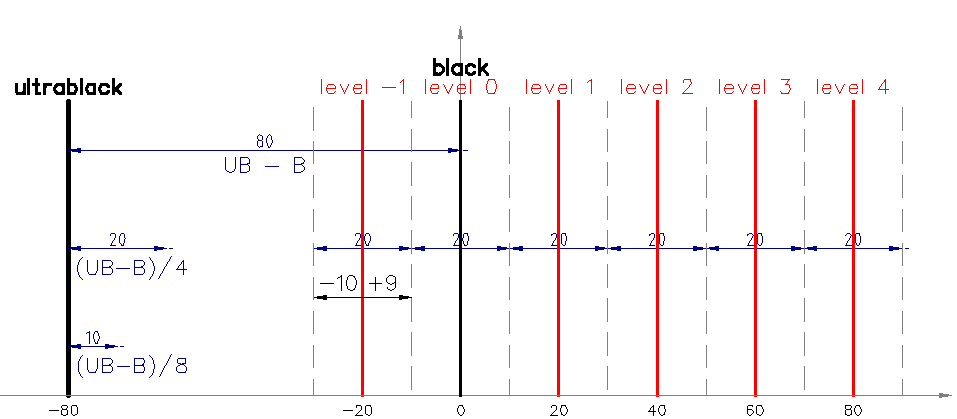
\includegraphics[width=0.95\textwidth]{decode}
	\caption{Schematic of the decoding. The red lines correspond to the ideal position of the level derived from the \ac{UB} and \ac{B}. If a measured value lies in between two dashed grey lines it will be decoded as that level.}
	\label{p15}
\end{figure}

% ========================================================
% 3
% ========================================================
\section{Pattern Generator}
The \ac{PG} is able to send out each of the four commands to the \ac{ROC}: a trigger, a  
\begin{wrapfigure}{r}{3.5cm}
	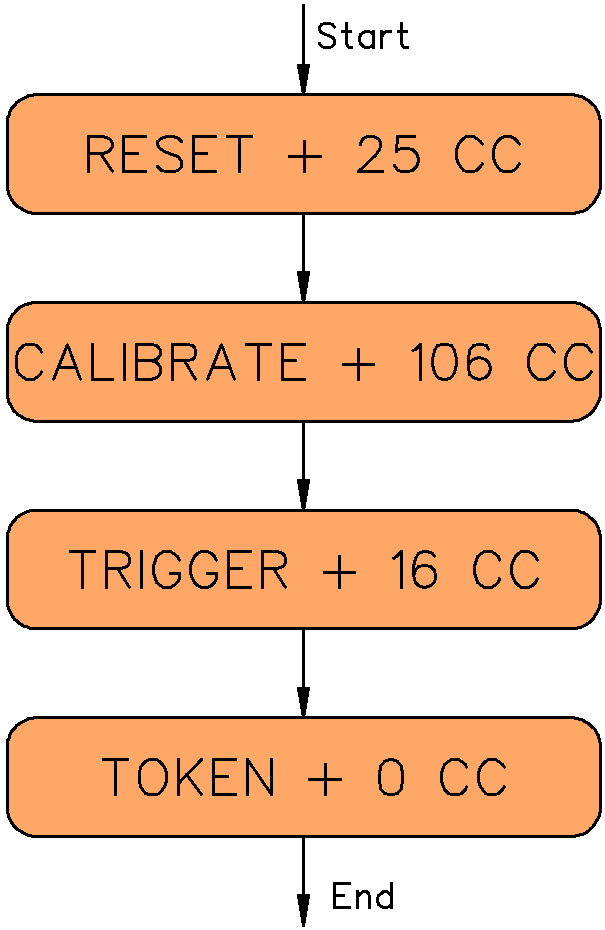
\includegraphics[width=3.4cm]{PG}
	\caption{example sequence of the \ac{PG}, CC stands for clock cycle}
	\label{p14}
\end{wrapfigure} 
token, a calibrate or a reset. A calibrate will sent out a calibration pulse to the \ac{ROC} and the reset basically deletes all hit information on the \ac{ROC}. It has a register bank with $256$ addresses at its disposal and each of these addresses can hold a single of the four commands and a delay. In that fashion there may be created arbitrary sequences of the four commands. Once the delay is set to $0$ the \ac{PG} will recognise this as a stop sign an ignore the rest of the sequence. An example is shown in \ar{p14}. This would be a basic set-up to test the functionality of the pixels. After a reset to delete all former hit information a calibrate is sent out. To read out the this event, the delay between trigger and calibrate has to be set to \textit{wbc}$+6$ to compensate for the duration the trigger needs to get to the \ac{ROC}. As the final step, the token is send out to collect the data.
% ========================================================
% 4
% ========================================================
\section{Python Interface}
Using cython most of the pXar-core functions are also accessible via python. All the available functions are listed in the cython header file \linebreak[4] ``PyPxarCore.pxd''. Should a function be amiss, it can be added to the header and the source file ``PyPxarCore.pyx`` just like in C++. So that the changes can come into effect and to use the PyPxarCore file the whole program has to be recompiled with the option ``python''.\\
Once that is done the already existing python \ac{CLI} interface ''cmdline.sh`` can be started, which initialises the \ac{DUT} in the same fashion as pXar would do it and allows to program and readout the \ac{DUT} with \ac{API}'s functions.
% ========================================================
% 4
% ========================================================
\section{Running the Software}
Once the software is properly installed meeting all the prerequisites, pXar needs a few configuration files to get started. For each \ac{ROC} that is connected to the \ac{DTB} pXar requires a file called ''dacParameters\_C$<$\ac{I2C}$>$.dat`` with all available \ac{DAC}s and corresponding start values for the respective \ac{ROC} and a file ''trimParameters\_$<$\ac{I2C}$>$.dat`` with a trim bit value for each pixel. If a completely untrimmed \ac{ROC} is required, all values have to be set to $15$, i.e. no trimming at all. Furthermore a file with delay settings for the \ac{DTB} called ''tbParameters.dat`` and a general configuration file ''configParameters.dat`` are required. Examples of these can be found in the appendix \ac{makelink}.\\
All the above files are mandatory to start the software and have to be in the same location (configuration directory). The binary files of pXar are in the directory bin of the installation folder. To run the software one has to go there and enter the command:
\begin{itemize}
	\item[$>$] ./pXar -d $<$configuration directory$>$
\end{itemize}
There are some further useful options to start the program that can be displayed using the ''-h`` option, but it will not start without ''-d``. To name the most important:
\begin{itemize}
	\item -f $<$flashfile$>$ \ka $\rightarrow$ flash a firmware from the flashfile to the \ac{FPGA} of the \ac{DTB}
	\item -g \ka $\rightarrow$ directly starts the \ac{GUI}
\end{itemize}
Since the software will start in a rather undocumented \ac{CLI} if started without the \ac{GUI} option, I recommend starting it always with the ``-g'' option as well.\\
For using the much more user specific \ac{CLI} I was always using the python version, which can be found in the python folder of the installation directory and starts with:
\begin{itemize}
	\item[$>$] ./cmdline.sh -d $<$configuration directory$>$
\end{itemize}
and is very powerful for performing and composing short tests and directly using the \ac{API} commands.
% ========================================================
% 5
% ========================================================
\section{EUDAQ}
EUDAQ is a \ac{DAQ} framework that was designed to be portable, modular and cross platform and was written in C++. It was mainly developed for the EUDET Pixel Telescope, but is very useful for other systems as well \cite{eudaq}. The program is split into different sub processes that can all run on different machines using \ac{TCP} sockets, which are shown in \ar{p16}.\\
The Run Control behaves like a central supervisor of the \ac{DAQ} and shows all the other connected processes, which is why it is the only process that has to run. All the hardware that is connected, e.g. the telescope, a \ac{TU} or other \ac{DUT}s, will have a Producer process and are thereby able to be configured, read out and to send the data to the Data Collector. The Data Collector collects the data from all Producers, combines it to a single data stream and saves it to native binary format. To keep track of potential errors there is also a Logger available that receives log messages from all processes, may receive messages from the user via the Run Control as well and saves the data in single location.\\
Thus, the reason for us using EUDAQ is quite obvious. It makes it very easy to use events off different producers and combine them into one data stream. Though there is still the urge for a trigger logic (q.v. \ar{makeref}) to keep all the events aligned. For the future the idea is to run with another Producer called \ac{TU} that can be configured in the same way as the whole trigger logic.\\
Being independent software, EUDAQ still uses the pXar-core library to operate the telescope.
\begin{figure}[ht]
	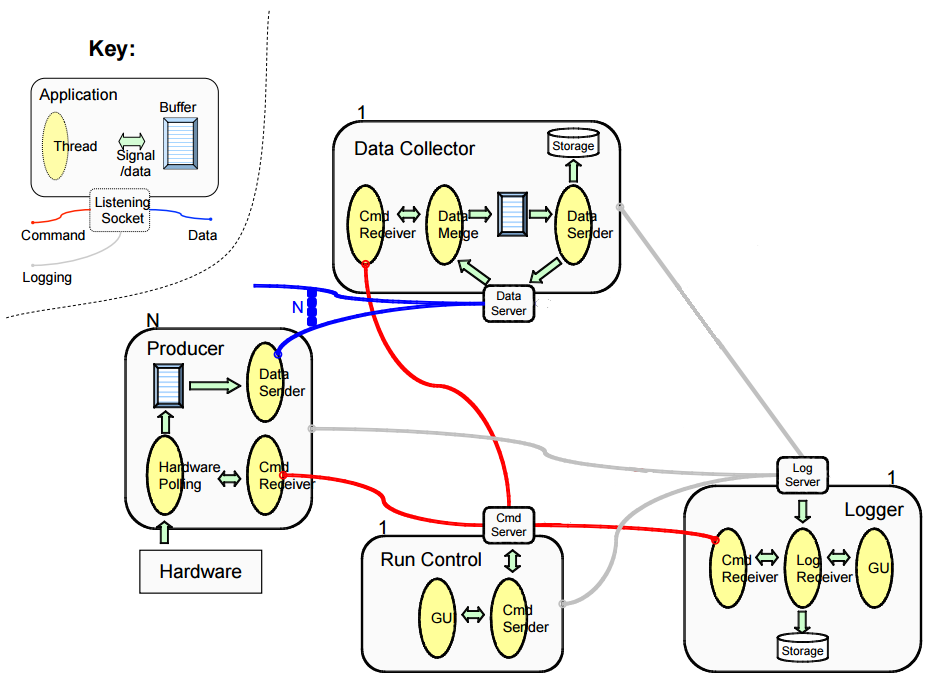
\includegraphics[width=0.95\textwidth]{eudaq}
	\caption{Schematic of the EUDAQ architecture \cite{eudaq}.}
	\label{p16}
\end{figure}

\chapter{Measurements}
\chapter{Analysis}
\chapter{Results}



% ========================================================
% ACRONYMS
% ========================================================
\chapter*{List of Acronyms}
\input{compile/acronyms.dat}
% ========================================================
% APPENDIX
% ========================================================
\appendix
\chapter{Dummy Appendix}

You can defer lengthy calculations that would otherwise only interrupt
the flow of your thesis to an appendix.

% ========================================================
% BIBLIOGRAPHY
% ========================================================
\backmatter
\bibliographystyle{plain}
\bibliography{compile/refs}
\includepdf[pages={-}]{declaration-originality.pdf}
% ============================
% DOCUMENT END
% ============================
\end{document}

